Nuestro algoritmo chequea en cada paso si existe alg\'un gimnasio capaz de ser vencido y, si existe, busca cual es el m\'as cercano, por lo tanto existir\'an casos en los cuales la soluci\'on obtenida para los mismos sea la \'optima pero para algunos no lo ser\'a.

\subsubsection*{Familias con soluci\'on obtenida igual a la \'optima}

%\begin{enumerate}
%\item No se obtiene soluci\'on por no haber las pokeparadas necesarias para ganar en todos los gimnasios.
%\item No se obtiene soluci\'on ya que la capacidad de la mochila no puede contener las pociones necesarias para vencer a un cierto gimnasio.
%\item Todos los gimnasios sin necesidad de pociones para ser vencidos.
%\item Las pokeparadas y los gimnasios se reciben en orden de la forma en la cual exista una pokeparada puntual para ir a cada gimnasio
%\end{enumerate}

\begin{center}
\textbf{Familia 1 y 2}
\end{center}

Ambas familias devolverán -1 ya que como se explicó anteriomente tanto el greedy como el exacto presentan podas para estos casos sin soluci\'on por lo tanto, su tiempo de ejecuci\'on ser\'a aproximadamente el mismo. \\\\

\begin{figure}[h]
 \centering
  \subfloat[Familia 1: actua poda 1]{
    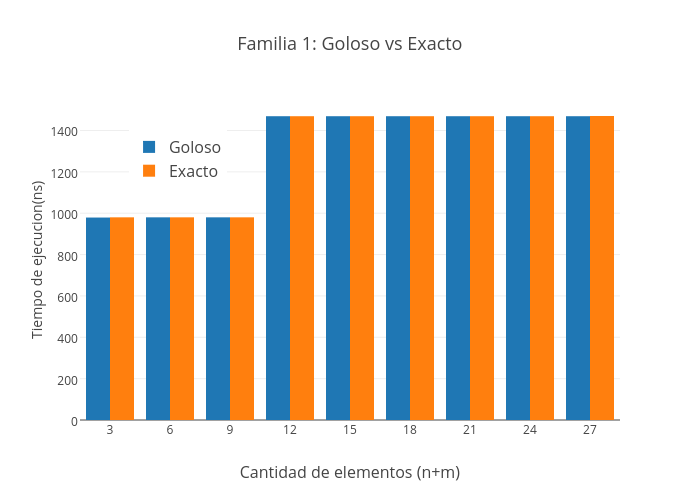
\includegraphics[width=0.45\textwidth]{./EJ2/fam1medicion.png}}
       \label{fig:fam1medicion}
  \subfloat[Familia 2: actua poda 2]{
    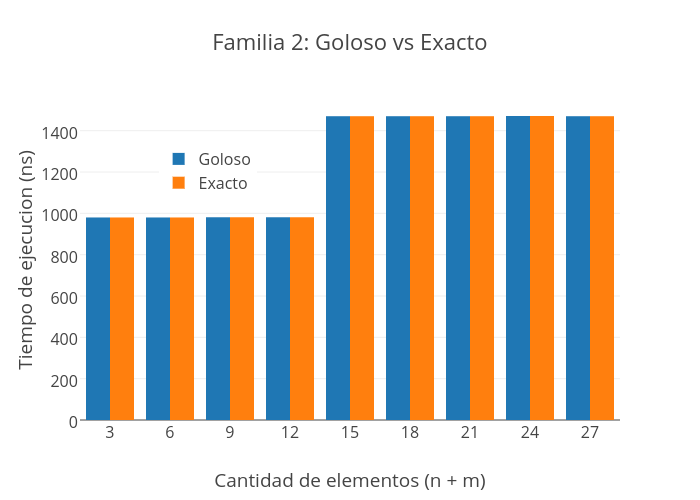
\includegraphics[width=0.45\textwidth]{./EJ2/fam2medicion.png}}
    \label{fig:fam2medicion}
    \end{figure}

Como se observa en los \'ultimos gr\'aficos, las funciones resultantes para cada familia en ambos algoritmos presentan el mismo tiempo por lo comentando sobre las podas realizadas.

\begin{center}
\textbf{Familia 3}
\end{center}

En este caso, como nuestro greedy chequea si hay alg\'un gimnasio a ser vencido con la cantidad de pociones que se tienen en el momento (se inicia con 0), y como todos necesitan 0, recorre los gimnasios sin necesidad de pasar por las pokeparadas, obteniendo la mejor soluci\'on posible.

A continuaci\'on mostraremos el camino obtenido tanto para el algoritmo exacto como el goloso de un caso en el que se trabaja con 8 elementos en total para ejemplificar lo enunciado anteriormente:

   \vspace*{0.3cm} \vspace*{0.3cm}
  \begin{center}
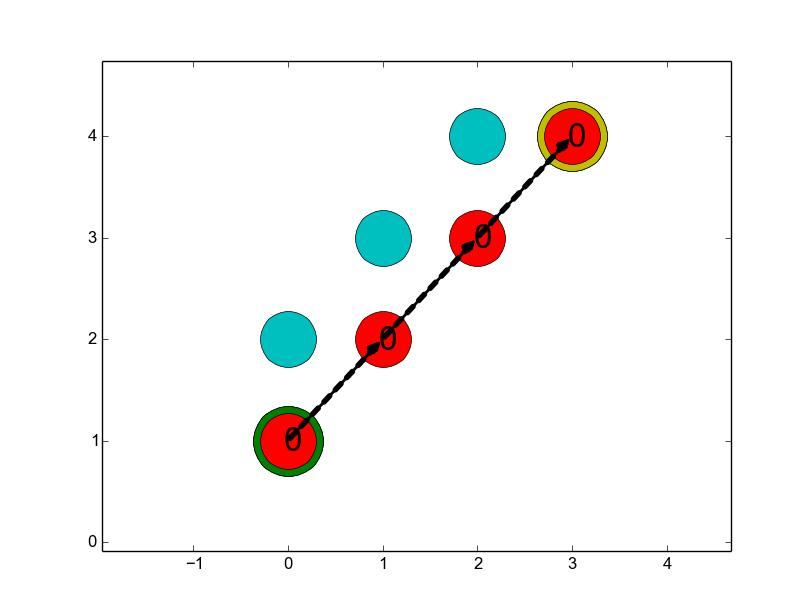
\includegraphics[scale=0.40]{./EJ2/todos0.png}
\\{\textit{Punteado = resultado exacto, contínua = resultado goloso}}
  \end{center}
  \vspace*{0.3cm}

Como se observa en el ejemplo el camino obtenido es exactamente el mismo.

\begin{center}
\textbf{Familia 5}
\end{center}

Se obtendr\'a la soluci\'on \'optima para esta familia ya que se reciben primero pokeparadas para vencer a un gimnasio cerca del mismo y luego m\'as pokeparadas para vencer a otros gimnasios que se encuentren cerca de los mismos. Se mostrar\'a a continuaci\'on un dibujo que ejemplifica lo dicho:

\vspace*{0.3cm} \vspace*{0.3cm}
  \begin{center}
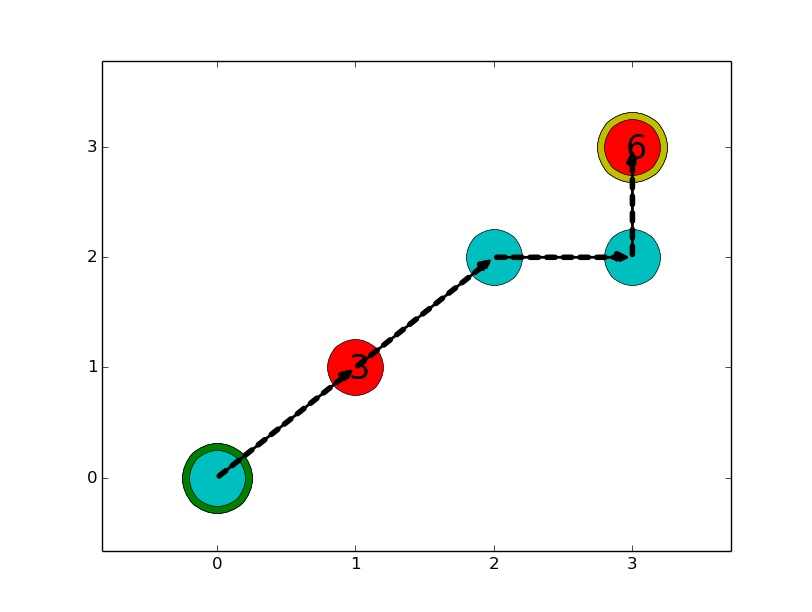
\includegraphics[scale=0.30]{./EJ2/optima.jpeg}
\\{\textit{Punteado = resultado exacto, contínua = resultado goloso}}
  \end{center}
  \vspace*{0.3cm}

\subsubsection*{Familia con soluci\'on no \'optima}

\begin{center}
\textbf{Familia 4}
\end{center}

En este tipo de familia existan gimnasios que no necesiten pociones para ser vencidos y otros que si. Nuestro algoritmo, por cada iteraci\'on chequea si puede elegir un gimnasio que se encuentre a una distancia m\'inima en relaci\'on a los demás, y adem\'as corrobora si posee las pociones necesarias para vencerlo, decide inicialmente ir a vencer a los gimnasios que posean cero poder, lo cual puede no ser \'optimo para el resultado final.

Este es un ejemplo del algoritmo exacto y el goloso con un total de 10 elementos:

\begin{figure} [!ht]
 \centering
  \subfloat[Algoritmo exacto]{
    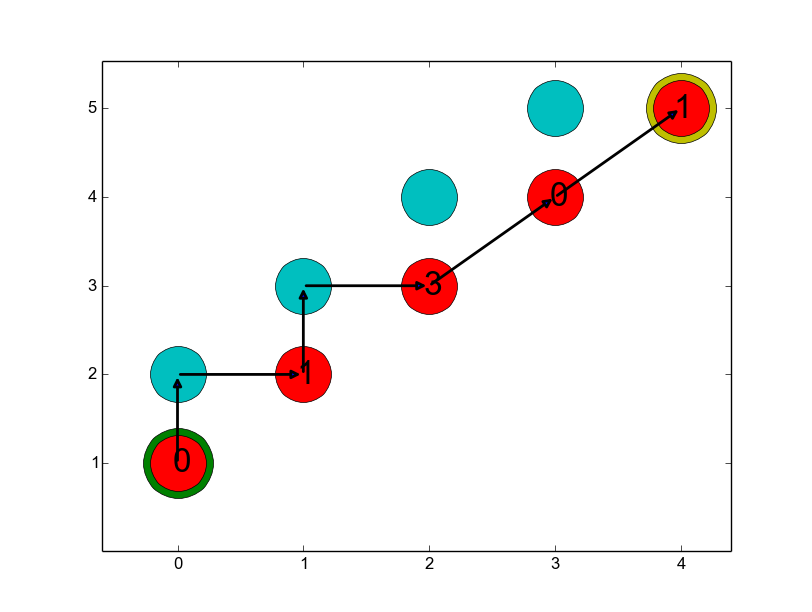
\includegraphics[width=0.45\textwidth]{./EJ2/fam5exacto.png}}
       \label{fig:fam5exacto}
  \subfloat[Algoritmo goloso]{
    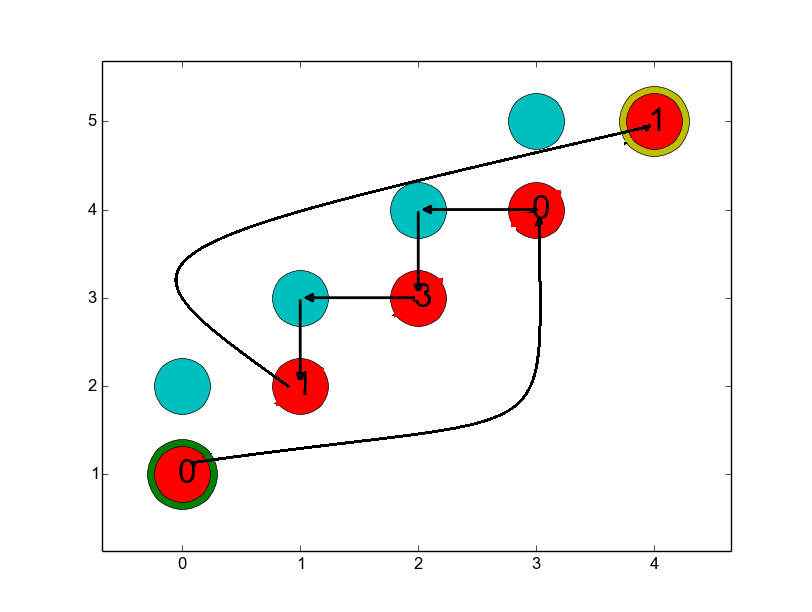
\includegraphics[width=0.45\textwidth]{./EJ2/fam5goloso.png}}
    \label{fig:fam5goloso}
    \end{figure}
    
Con respecto a la diferencia entre la soluciones que se obtienen en relacion a las óptimas elebaramos las siguientes comparaciones:\\\\
 

  \begin{figure} [h]
 \centering
  \subfloat[Comparación de distancias obtenidas]{
    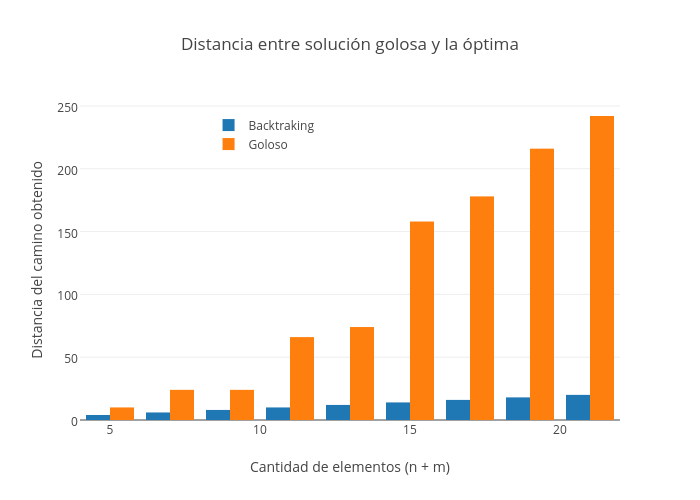
\includegraphics[width=0.5\textwidth]{./EJ2/gym0Dif.png}
    \label{fig:comparativo31}}
  \subfloat[Porcentaje de error relativo del goloso]{
    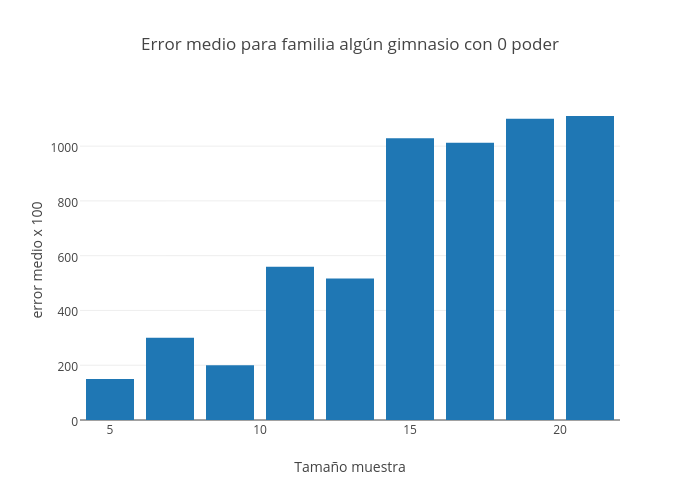
\includegraphics[width=0.5\textwidth]{./EJ2/gym0Error.png}
    \label{fig:comparativo32}}
    \end{figure} 
 
Debido al poder de cómputo utilizado para realizar los tests, solo pudo testearse el algoritmo exacto hasta con 20 elementos teniendo que bajar inclusive hasta 15 elementos para algunas familias, mientras que el goloso puede tomar una mayor cantidad de elementos con tiempos de ejecución considerablemente menores.

\begin{center}
\textbf{Familia 6}
\end{center}

Este estilo de familia presenta a los gimnasios y pokeparadas desordenados en referencia a las posiciones, es decir, para ganar a cierto gimnasio es necesario pasar por una cantidad puntual de pokeparadas las cuales estan de un lado y del otro de dicho gimnasio.
\\\\

  \begin{figure} [h]
 \centering
  \subfloat[Comparación de distancias obtenidas]{
    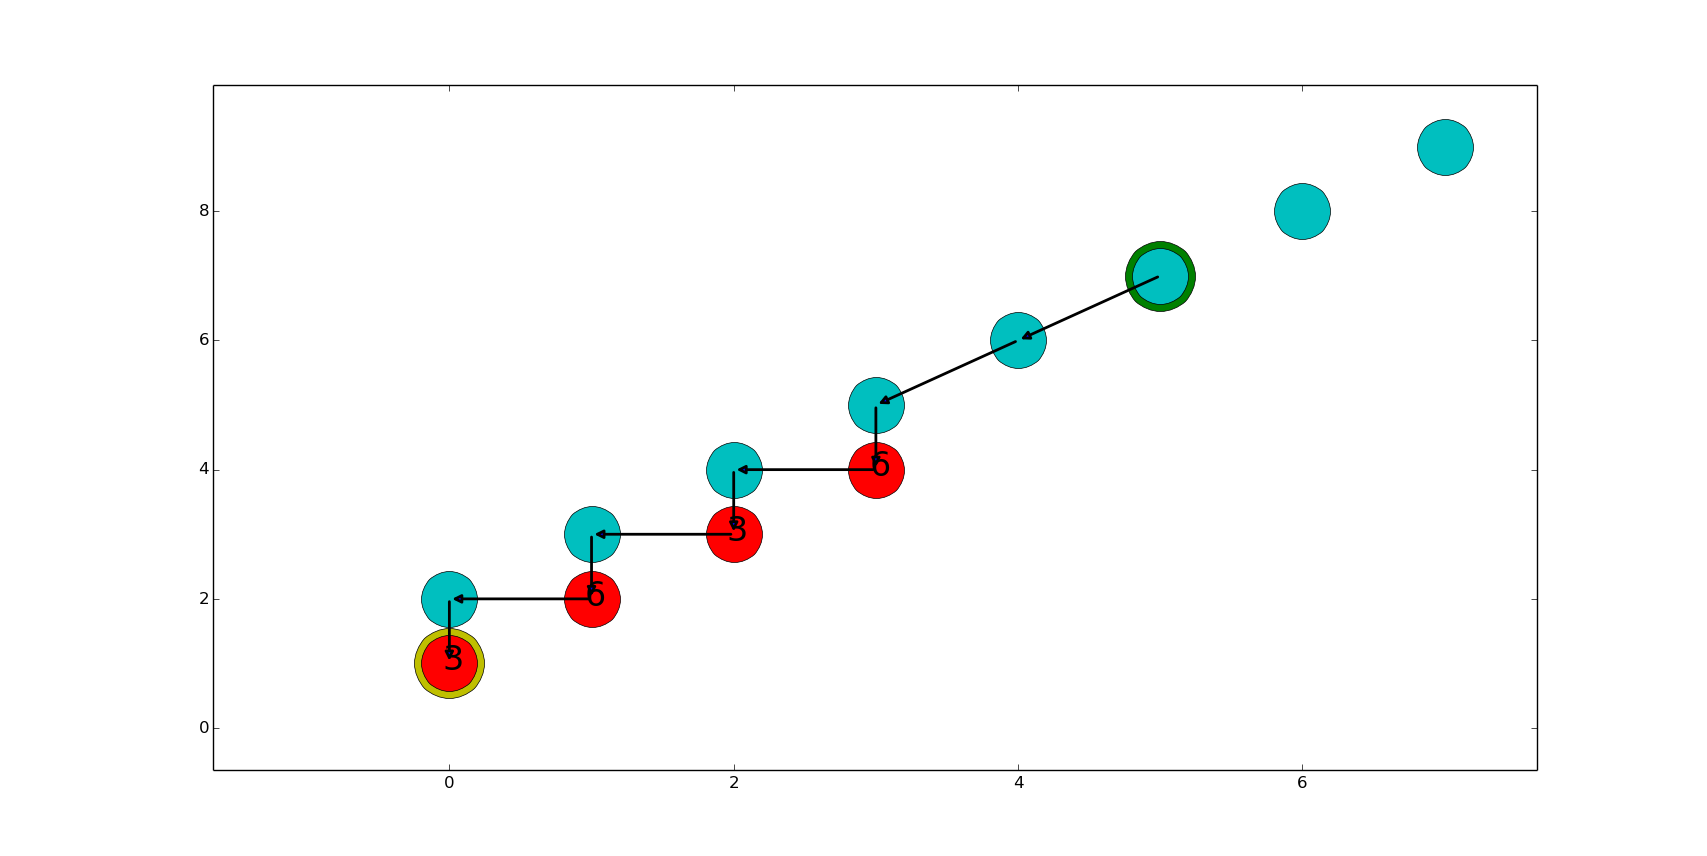
\includegraphics[width=0.50\textwidth]{./EJ2/caminosinorden1.png}
    \label{fig:caminosinorden1}}
  \subfloat[Porcentaje de error relativo del goloso]{
    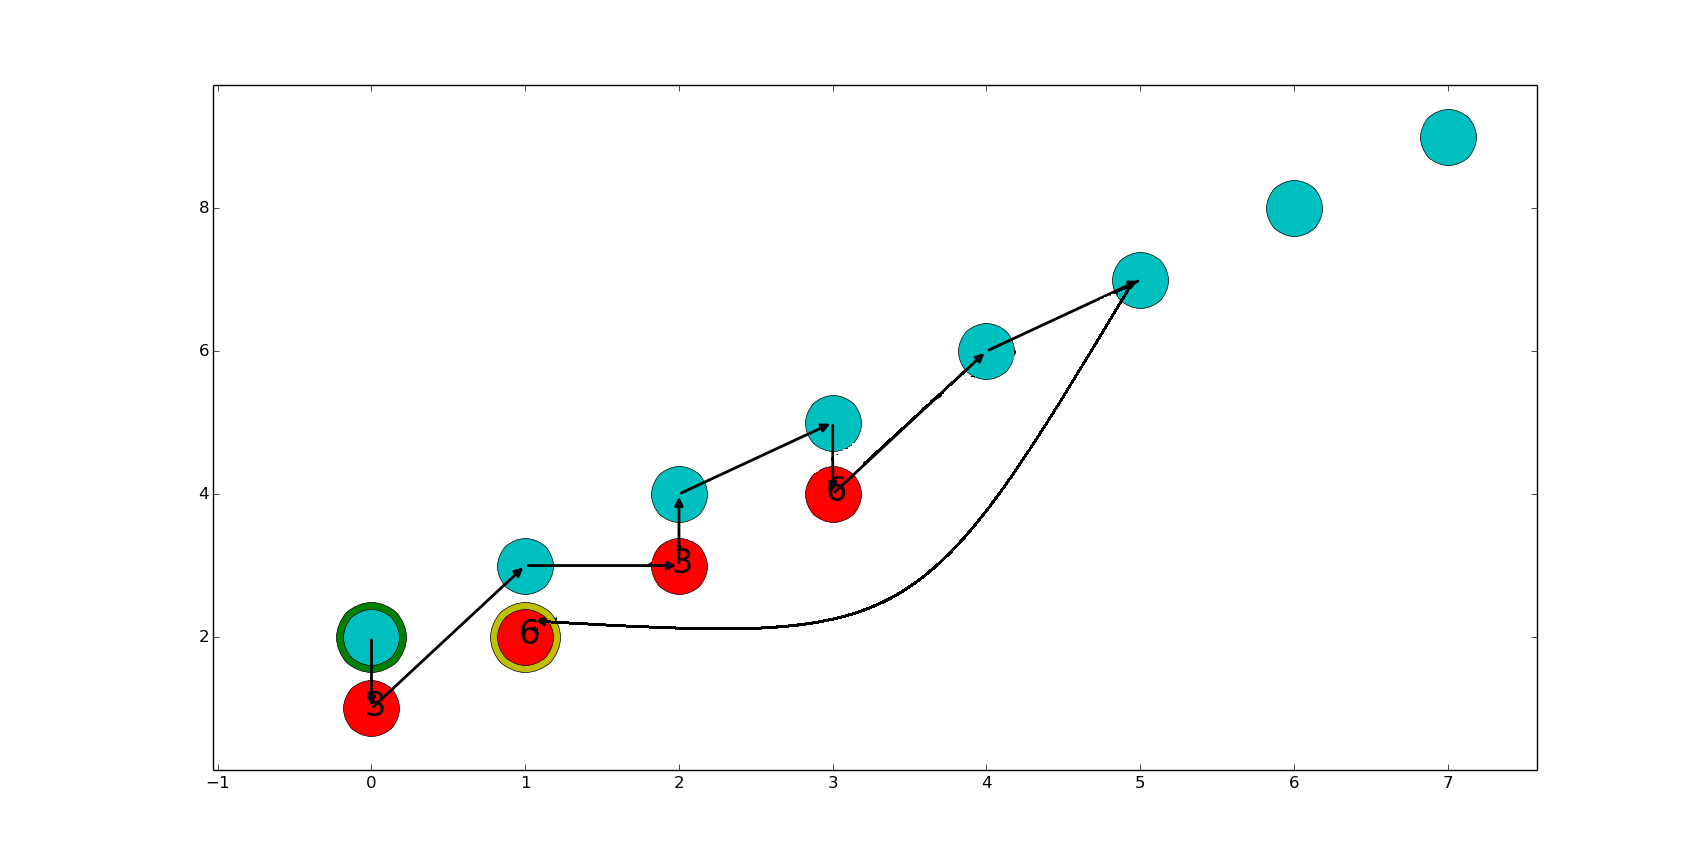
\includegraphics[width=0.50\textwidth]{./EJ2/caminosinorden.png}
    \label{fig:caminosinorden}}
    \end{figure} 

Se puede observar en el ejemplo como nuestro algoritmo goloso va a la primer pokeparada y de ah\'i a vencer al gimnasio m\'as cercano en vez de ir a la pokeparada consecutiva. Esto lo hace hasta vencer a todos los gimnasios.

La diferencia entre soluciones se pueden apreciear en los siguientes gràficos:\\

  \begin{figure} [h]
 \centering
  \subfloat[Comparación de distancias obtenidas]{
    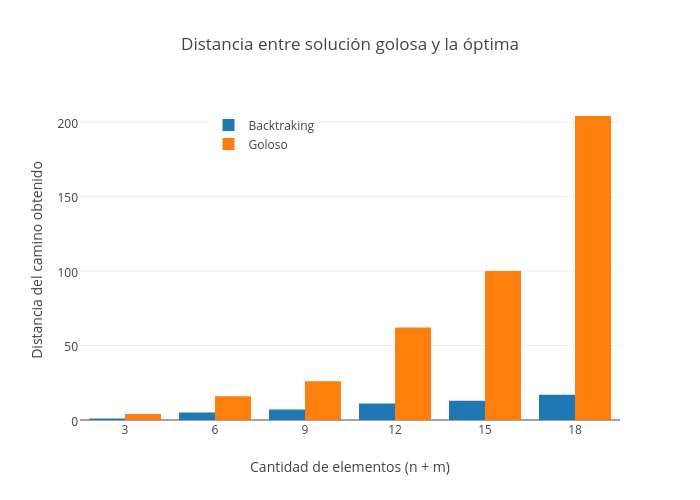
\includegraphics[width=0.50\textwidth]{./EJ2/sinOrdenDif.png}
    \label{fig:comparativo31}}
  \subfloat[Porcentaje de error relativo del goloso]{
    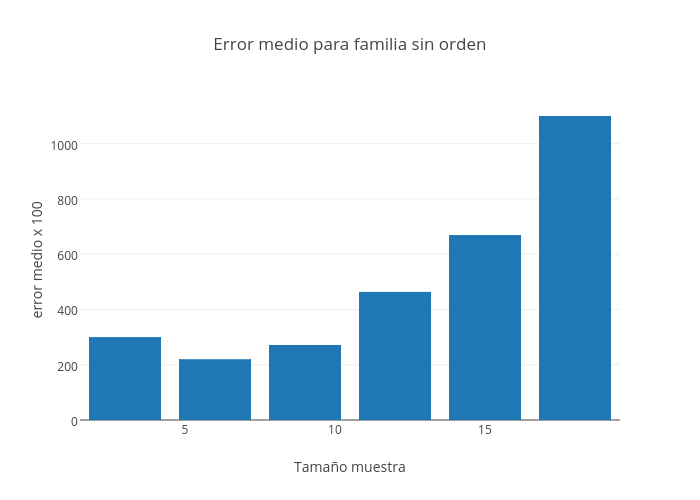
\includegraphics[width=0.50\textwidth]{./EJ2/sinordenError.png}
    \label{fig:comparativo32}}
    \end{figure} 

\begin{center}
\textbf{Familia 7}
\end{center}

El objetivo de esta familia es plantear un caso en donde, de forma controlada, la respuesta del algoritmo goloso nunca fuera la óptima. Para ello, se genera una instancia agrupando los gimnasios y pokeparadas en 2 anillos de radios diferentes. Dado que nuestro algoritmo siempre y cuando pueda vencer a alg\'un gimnasio buscará el m\'inimo en  distancia para vencerlo, para esta familia resultará contraproducente: es preferible adquirir m\'as pociones para luego ir a varios gimnasios juntos, que ganar apenas exista la posibilidad.

\newpage

\vspace*{0.3cm} \vspace*{0.3cm}
\begin{figure} [!ht]
 \centering
  \subfloat[Algoritmo exacto]{
    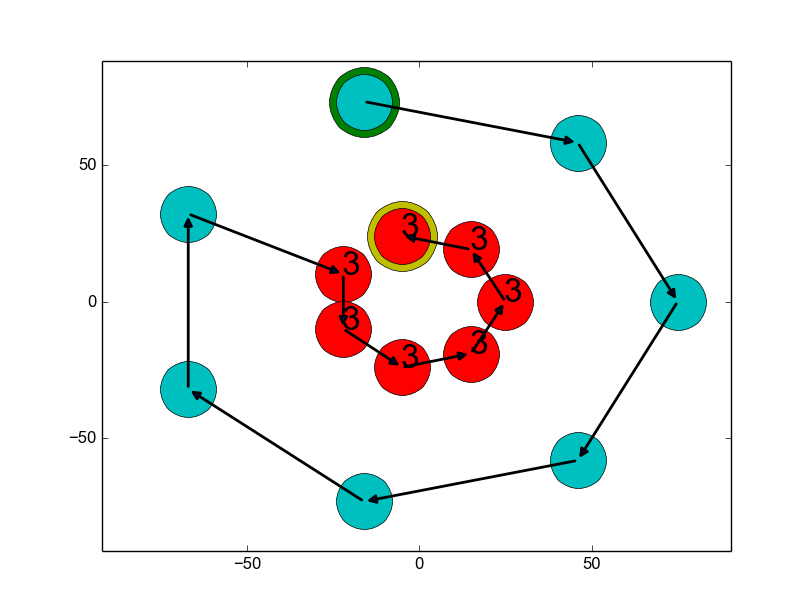
\includegraphics[width=0.45\textwidth]{./EJ2/anilloexacto.png}}
       \label{fig:anilloexacto}
  \subfloat[Algoritmo goloso]{
    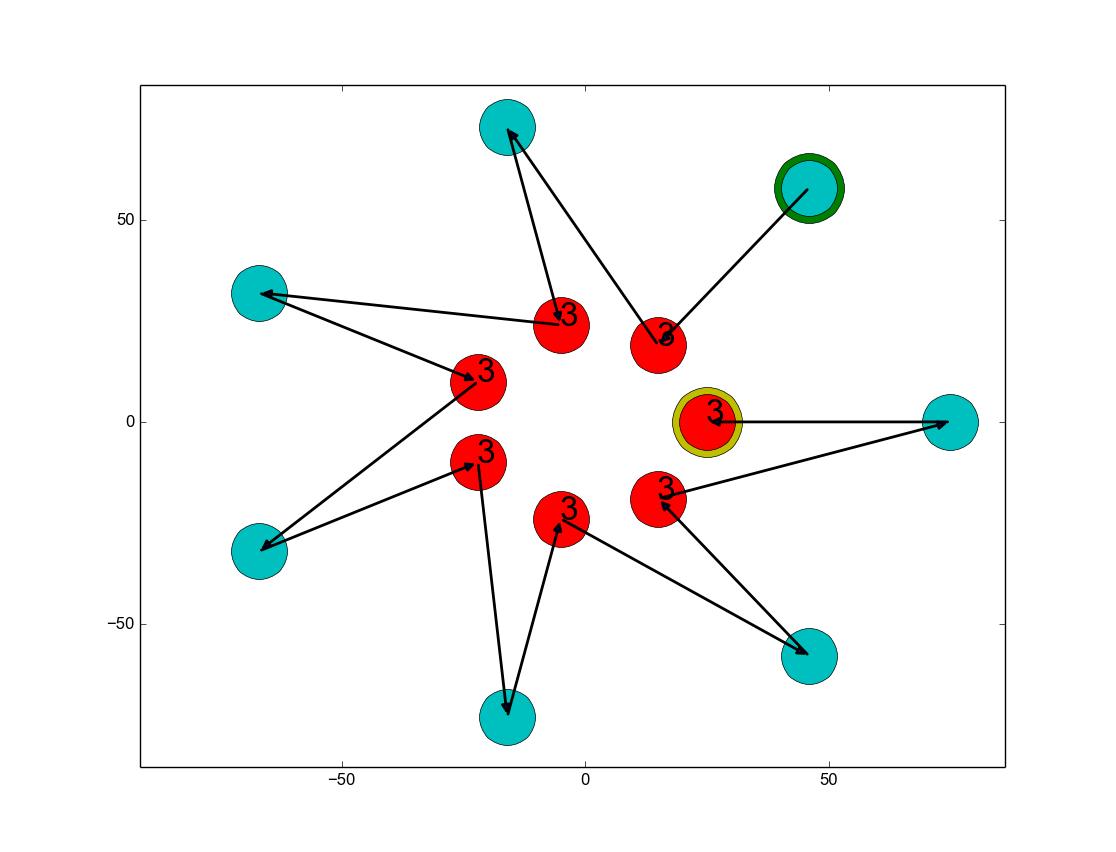
\includegraphics[width=0.45\textwidth]{./EJ2/anillogoloso.png}}
    \label{fig:anillogoloso}
    \end{figure}
\vspace*{0.3cm} \vspace*{0.3cm}

Se puede observar en el \'ultimo gr\'afico como los resultados tienen valores diversos para casos pequeños. En las instancias de mayor tamaño, las solución óptima resulta de recorrer primero todas las pokeparadas y luego los gimnasios, ya que la cantidad de pociones necesarias para vencer a todos los gimnasios es igual a la cantidad total de pociones presentes en el mapa, sumado a que la distancia entre pokeparadas es muy inferior que entre pokeparadas y gimnasios.

Al generarse un camino alternado para el goloso entre gimnasio y pokeparada, se le dan a todos los gimnasios la dificultad igual a la cantidad de pociones que aporta cada pokeparada y se crean la misma cantidad de gimnasios como de pokeparadas. En cuanto a la distribución de los mismos, se buscó una forma de estrella, en la cual cada pokeparada está alineada con 2 gimnasios y una segunda pokeparada. Dadas estas restricciones se observa lo siguiente:

\vspace*{0.3cm} \vspace*{0.3cm}
  \begin{center}
 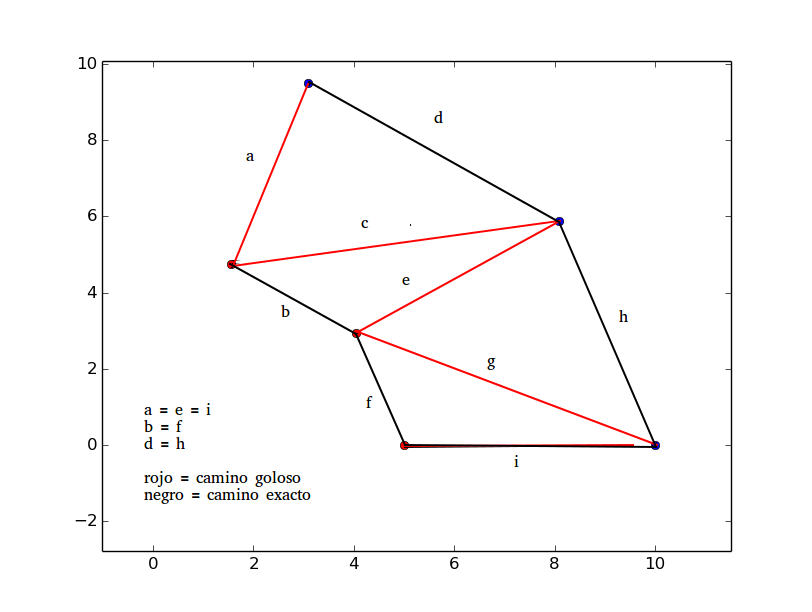
\includegraphics[width=0.75\textwidth]{./EJ2/dibujoorientativo.png}
\\{\textit{Comparación solución golosa vs exacta}}
  \end{center}

El camino goloso realiza un camino de longitud $\sum^{k}_{i=1}a + \sum^{j}_{i=1}c$ y el exacto $\sum^{n-1}_{i=1}b + \sum^{m-1}_{i=1}d + a$. Siendo $k$ el número de aristas como $a$ y $j$ como $c$, se tiene que $k + j = n+m-1$ (aristas en un camino de n+m elementos) y que $k=j+1$. Para que el algoritmo goloso difiera del exacto, se debe cumplir entonces la siguiente desigualdad:
\[
\sum^{k}_{i=1}a + \sum^{j}_{i=1}c \ge \sum^{n-1}_{i=1}b + \sum^{m-1}_{i=1}d + a
\]

La cual equivale a decir:

\[
\sum^{k}_{i=1}a + \sum^{j}_{i=1}c - a \ge (n-1)b + (m-1)d
\]

\[
\sum^{j}_{i=1}a + \sum^{j}_{i=1}c \ge (n-1)b + (m-1)d
\]

\[
j(a + c)\ge (n-1)b + (m-1)d
\]

Siendo que $n=m$ por como se construye la instancia, entonces:


\[
j(a + c) \ge (n-1)(b + d)
\]

Finalmente, como $k = j + 1 \wedge k+j=n+m-1 \leftrightarrow j = n - 1 $, se resolverán distintos caminos siempre y cuando $a +c \ge b + d$. Con lo cual, para generar correctamente las instancias para esta famila, se considero dicha desigualdad.

Podemos ver un ejemplo de la desigualdad de las soluciones presentes en las siguientes instancias corridas con el algoritmo goloso y el backtraking:
 
 
\vspace*{0.3cm} \vspace*{0.3cm}
\begin{figure} [!ht]
 \centering
  \subfloat[Algoritmo exacto]{
 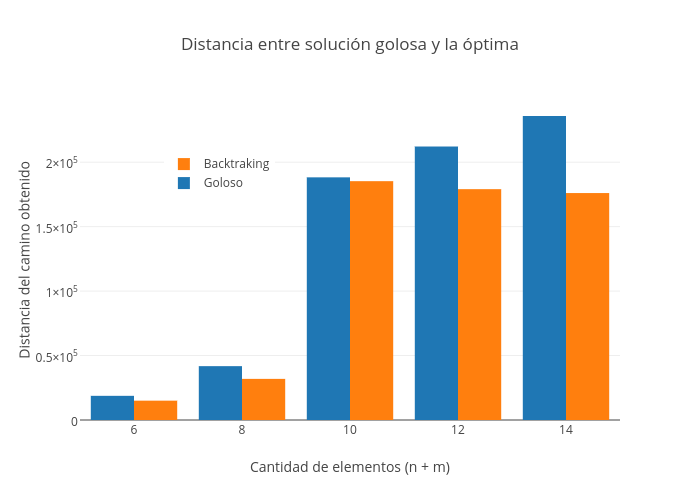
\includegraphics[width=0.5\textwidth]{./EJ2/anillosDif.png}
       \label{fig:anilloexacto}}
  \subfloat[Algoritmo goloso]{
   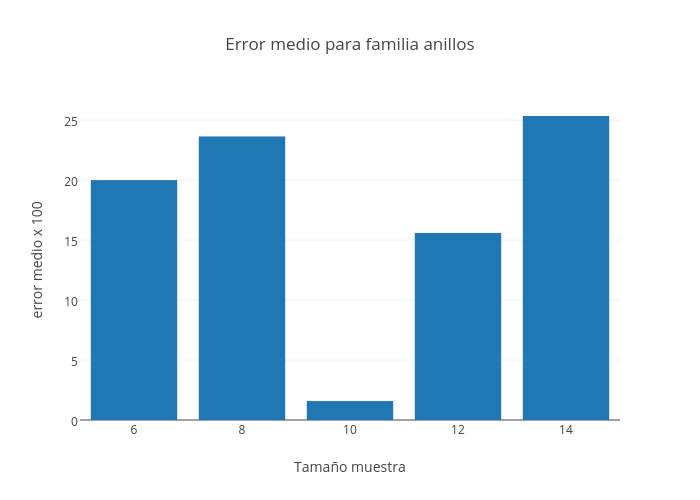
\includegraphics[width=0.5\textwidth]{./EJ2/anillosError.png}
    \label{fig:anillogoloso}}
    \end{figure}

 
Los radios para entradas de hasta 8 elementos son distintos al resto de las instancias. En síntesis se puede ver para los tamaños de 10 a 14 elementos que se mantuvo la distancia recorrida en el algoritmo exacto: esto se debe al carácter del camino, que resulta de recorrer primero una circunferencia, luego dirigirse de forma recta a la circunferencia interior y recorrerla. Al no haber variabilidad en los radios, el tiempo insumido es aproximadamente el mismo. No así para el algoritmo goloso, ya que un incremento en la cantidad de elementos, conyeva un incremento de las idas y vueltas a realizar; aumentando notoriamente la distancia del recorrido.


\subsubsection*{Comparación entre errores de familias}

Teniendo un grupo de familias que provocan soluciones con errores al aplicar el algoritmo goloso, podemos ver lo siguiente entre la Familia 4 y la Familia 6:

\vspace*{0.3cm} \vspace*{0.3cm}
  \begin{center}
 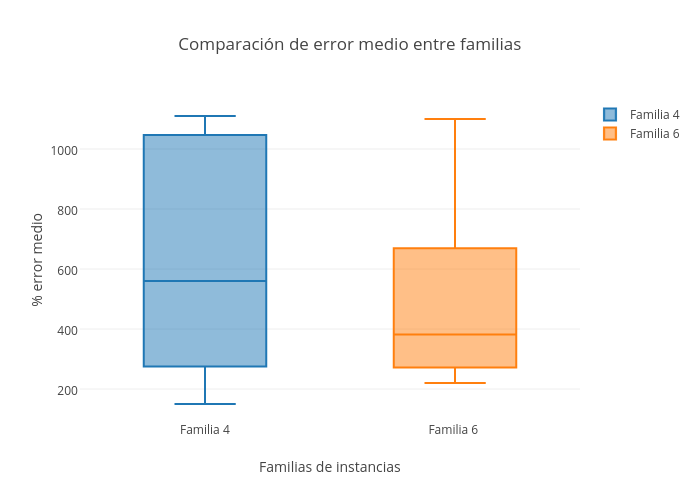
\includegraphics[width=0.75\textwidth]{./EJ2/box.png}
\end{center}

Se evidencia el mejor desempeño del algoritmo sobre la familia 6, provocando un error medio mucho menor que la familia 4 (alrrededor de 110\% mejor) y con una dispersión del mismo mucho más baja. 

De forma separada, debido a los rangos que se manejan, se decidió analizar la distribución de la Familia 7. Vale destacar que el error de la misma es muy inferior al de las dos anteriores y posee la menor varianza de todas. Esto se debe al carácter controlado de la misma, y su característica de posicionamiento: 
\vspace*{0.3cm} \vspace*{0.3cm}
  \begin{center}
 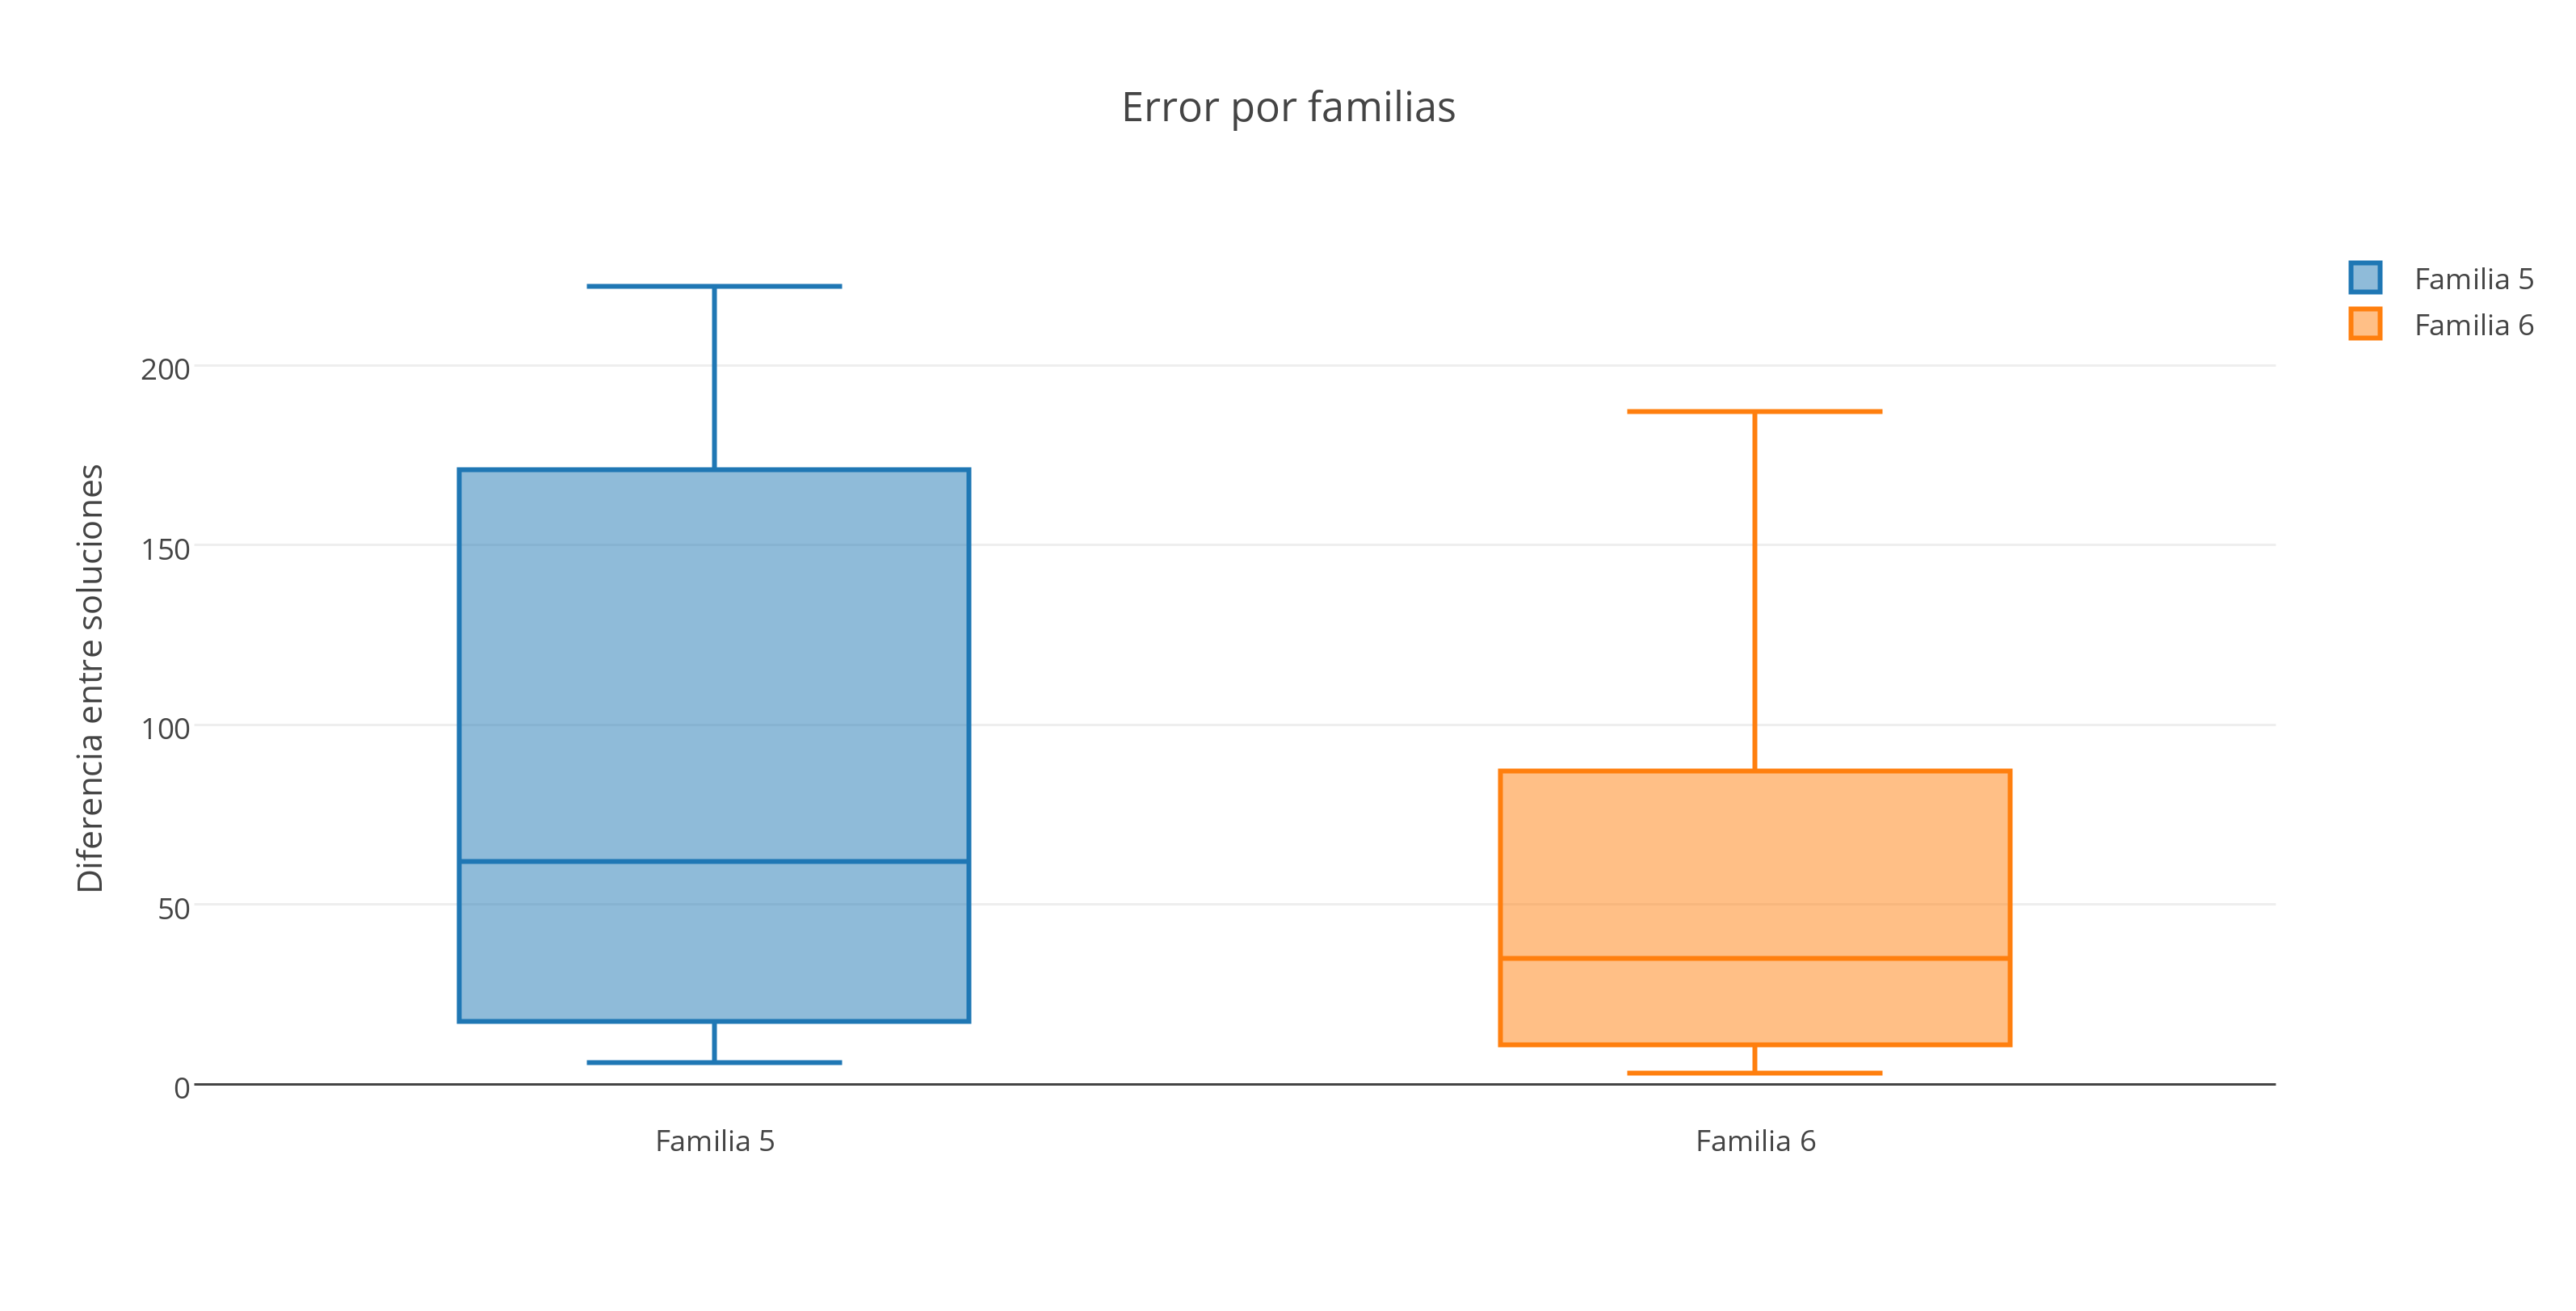
\includegraphics[width=0.75\textwidth]{./EJ2/box1.png}
\end{center}

\subsubsection*{Comparación entre tiempos de familias}

Veremos como se comporta cada familia en funci\'on del tiempo al ir aumentando la cantidad de elementos manteniendo las condiciones para que sigan perteneciendo cada uno a su respectiva familia.

\vspace*{0.3cm} \vspace*{0.3cm}
  \begin{center}
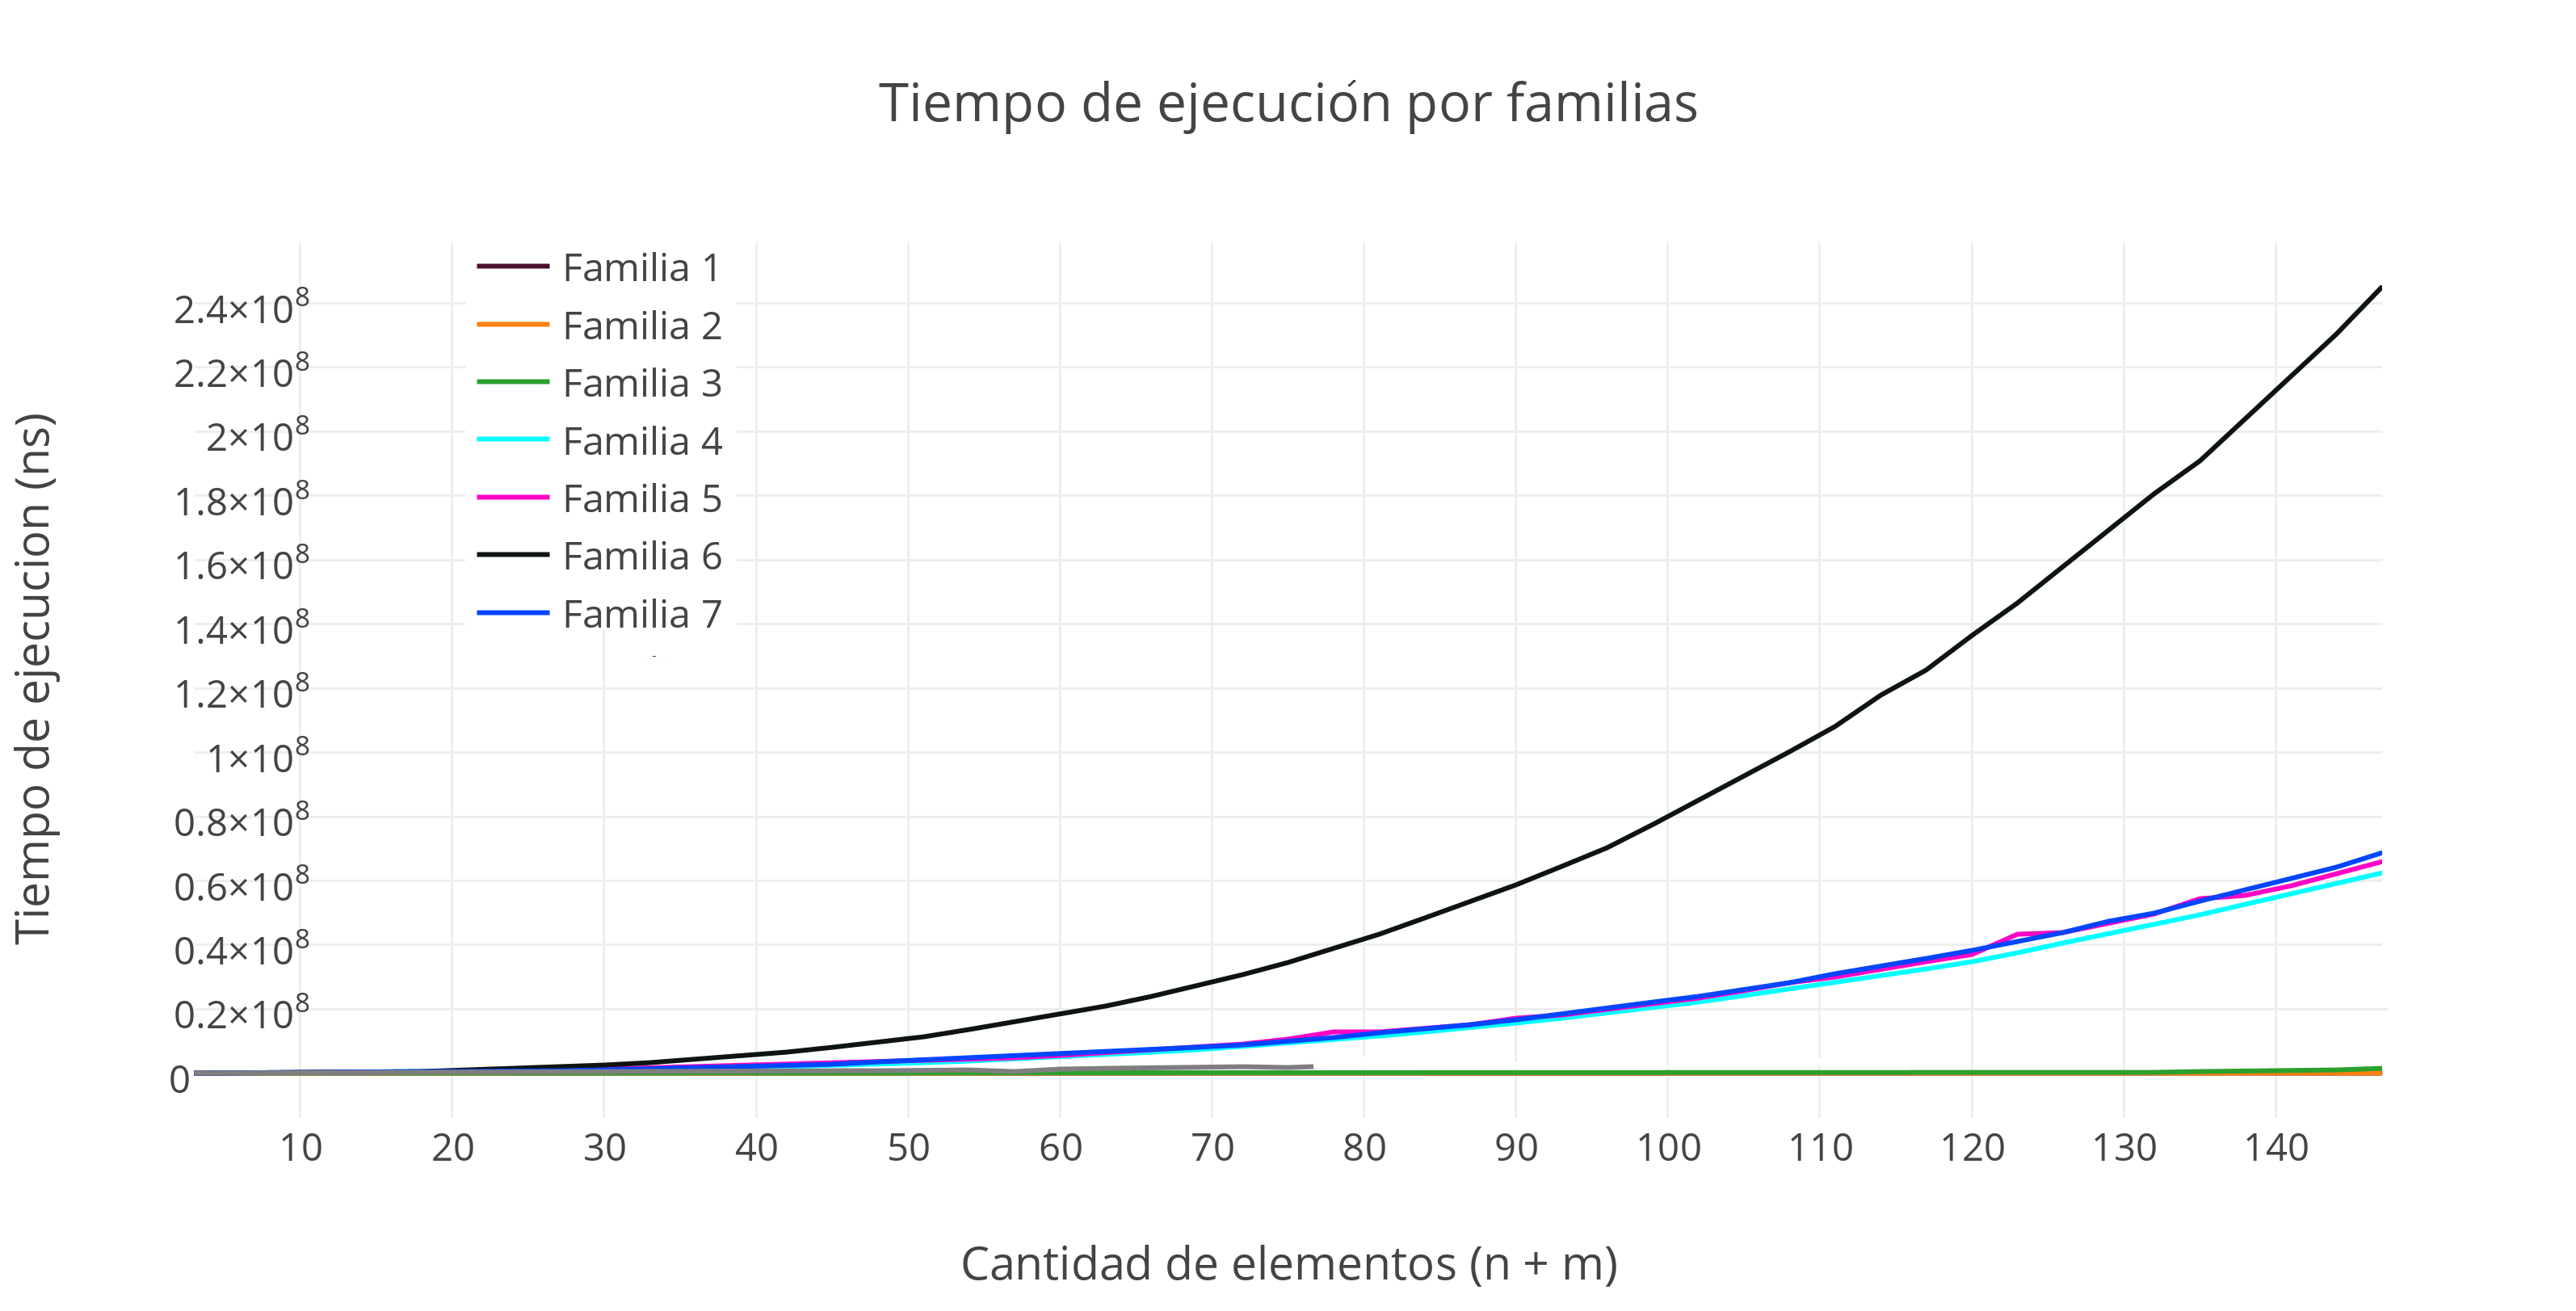
\includegraphics[scale=0.60]{./EJ2/comparativo.png}
\\{\textit{Tiempo de ejecución entre familias}}
  \end{center}
  \vspace*{0.3cm}
  \begin{figure} [!ht]
 \centering
  \subfloat[Detalle sin la familia 6]{
    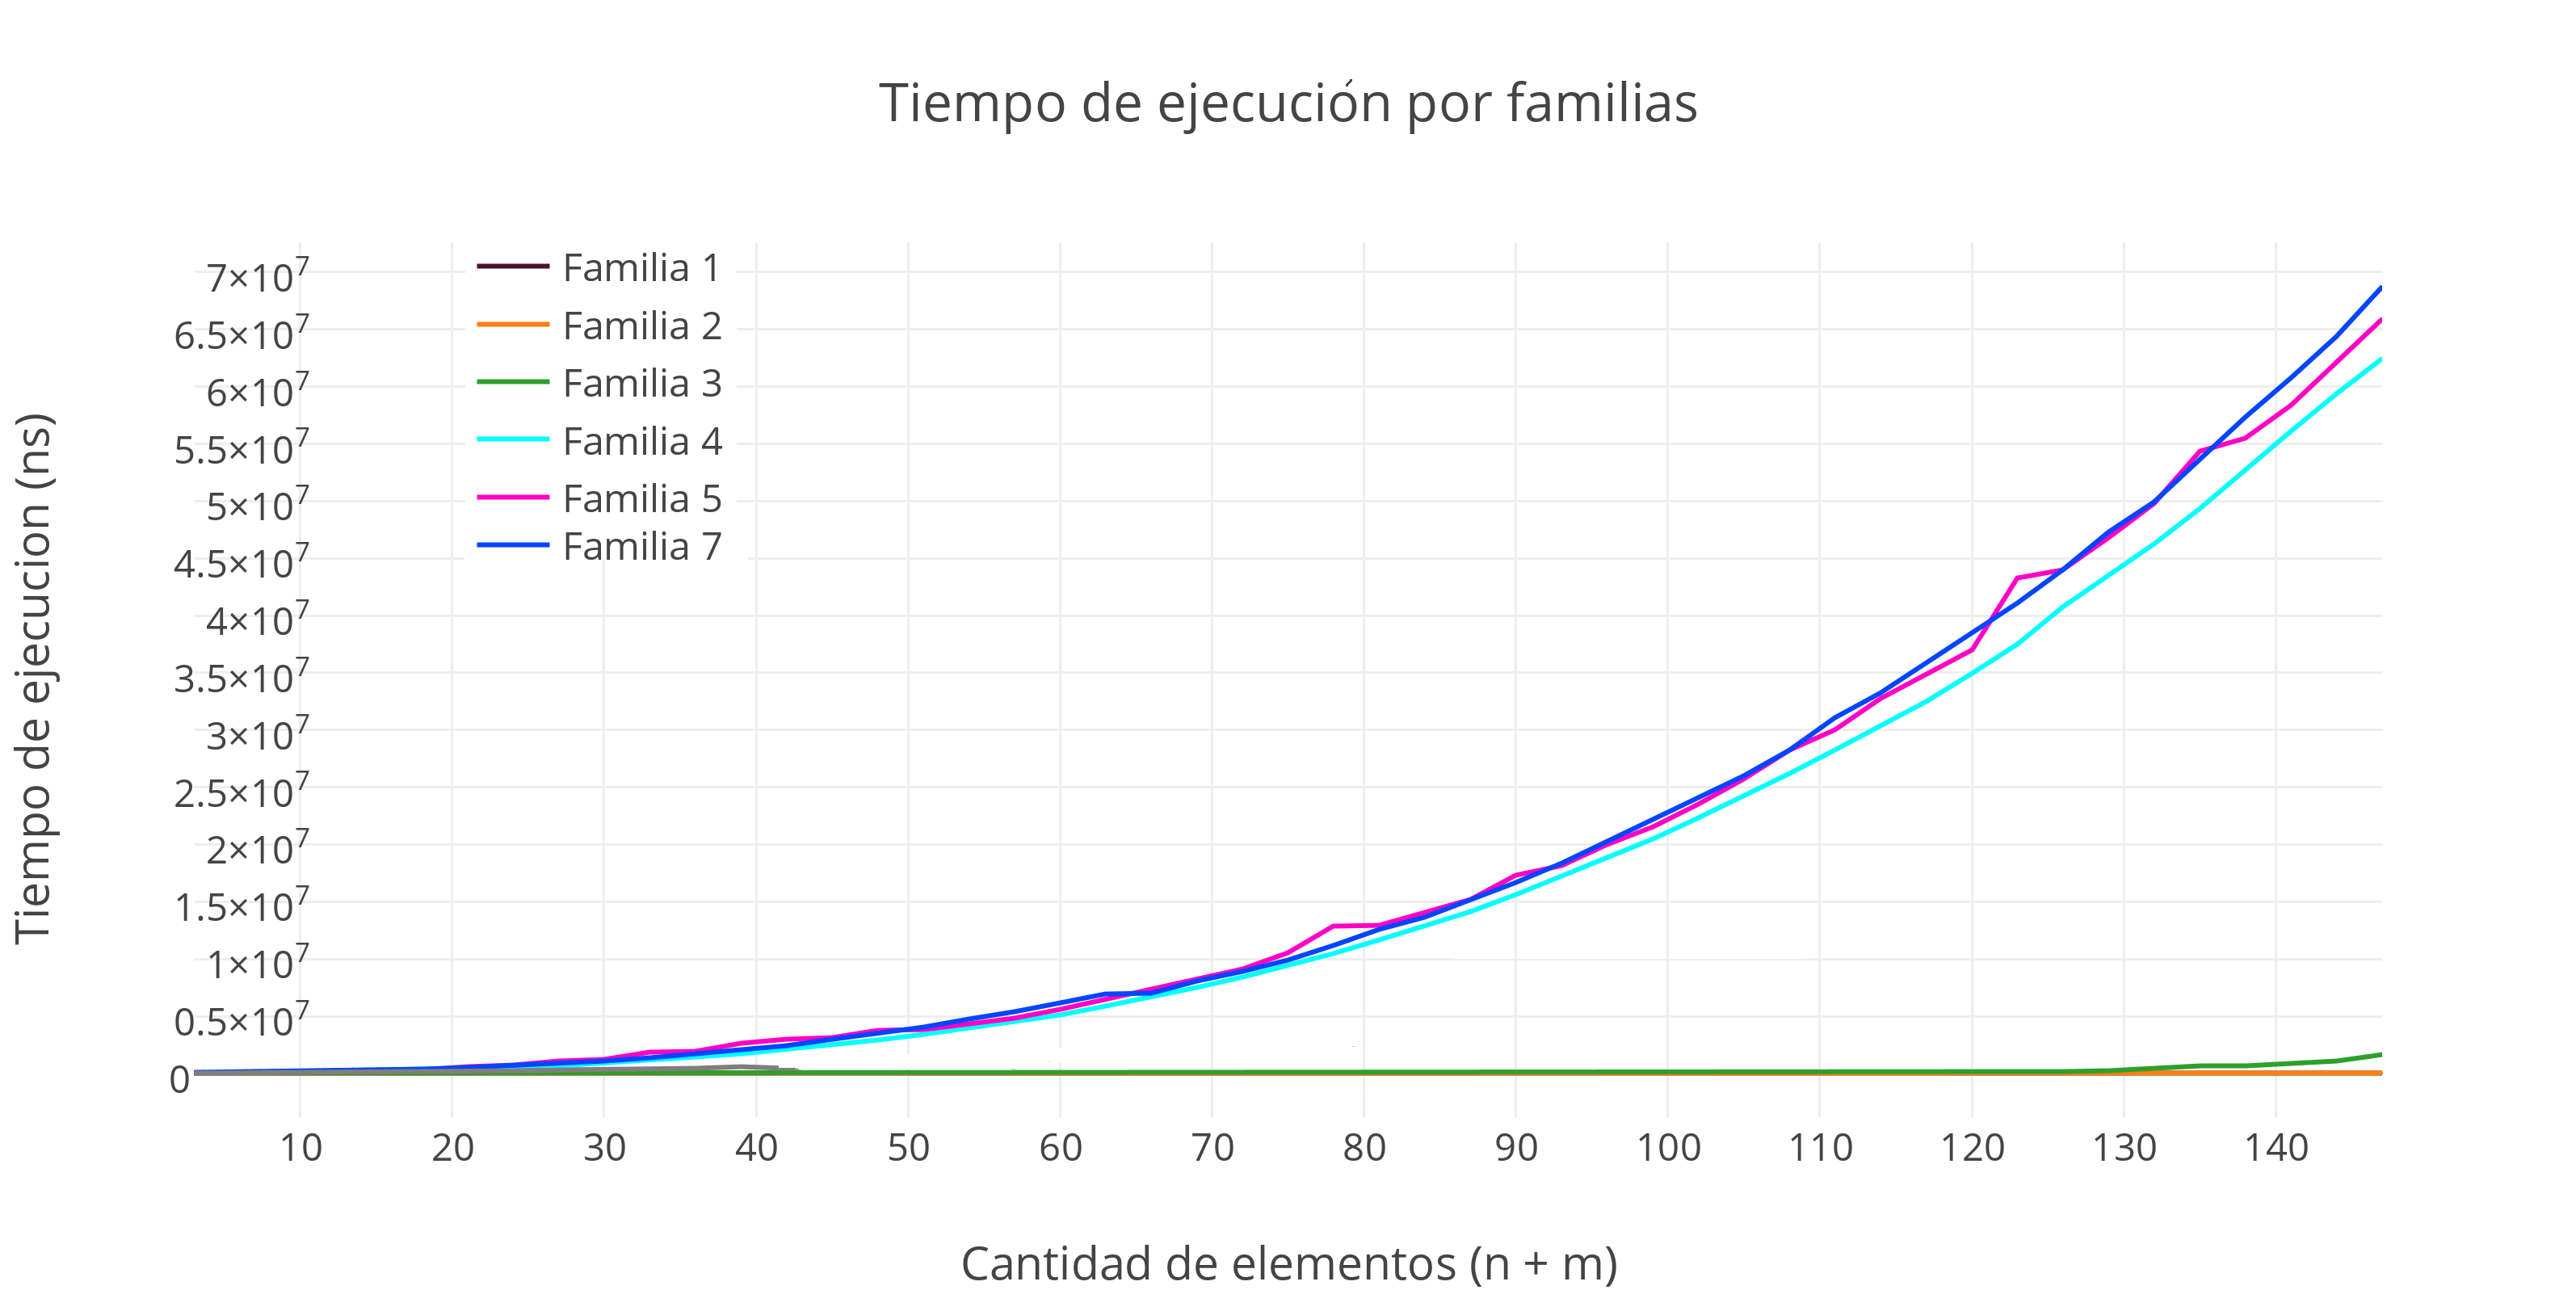
\includegraphics[width=0.45\textwidth]{./EJ2/comparativo1.png}}
    \label{fig:comparativo1}
  \subfloat[Detalle de las familias menos costosas]{
    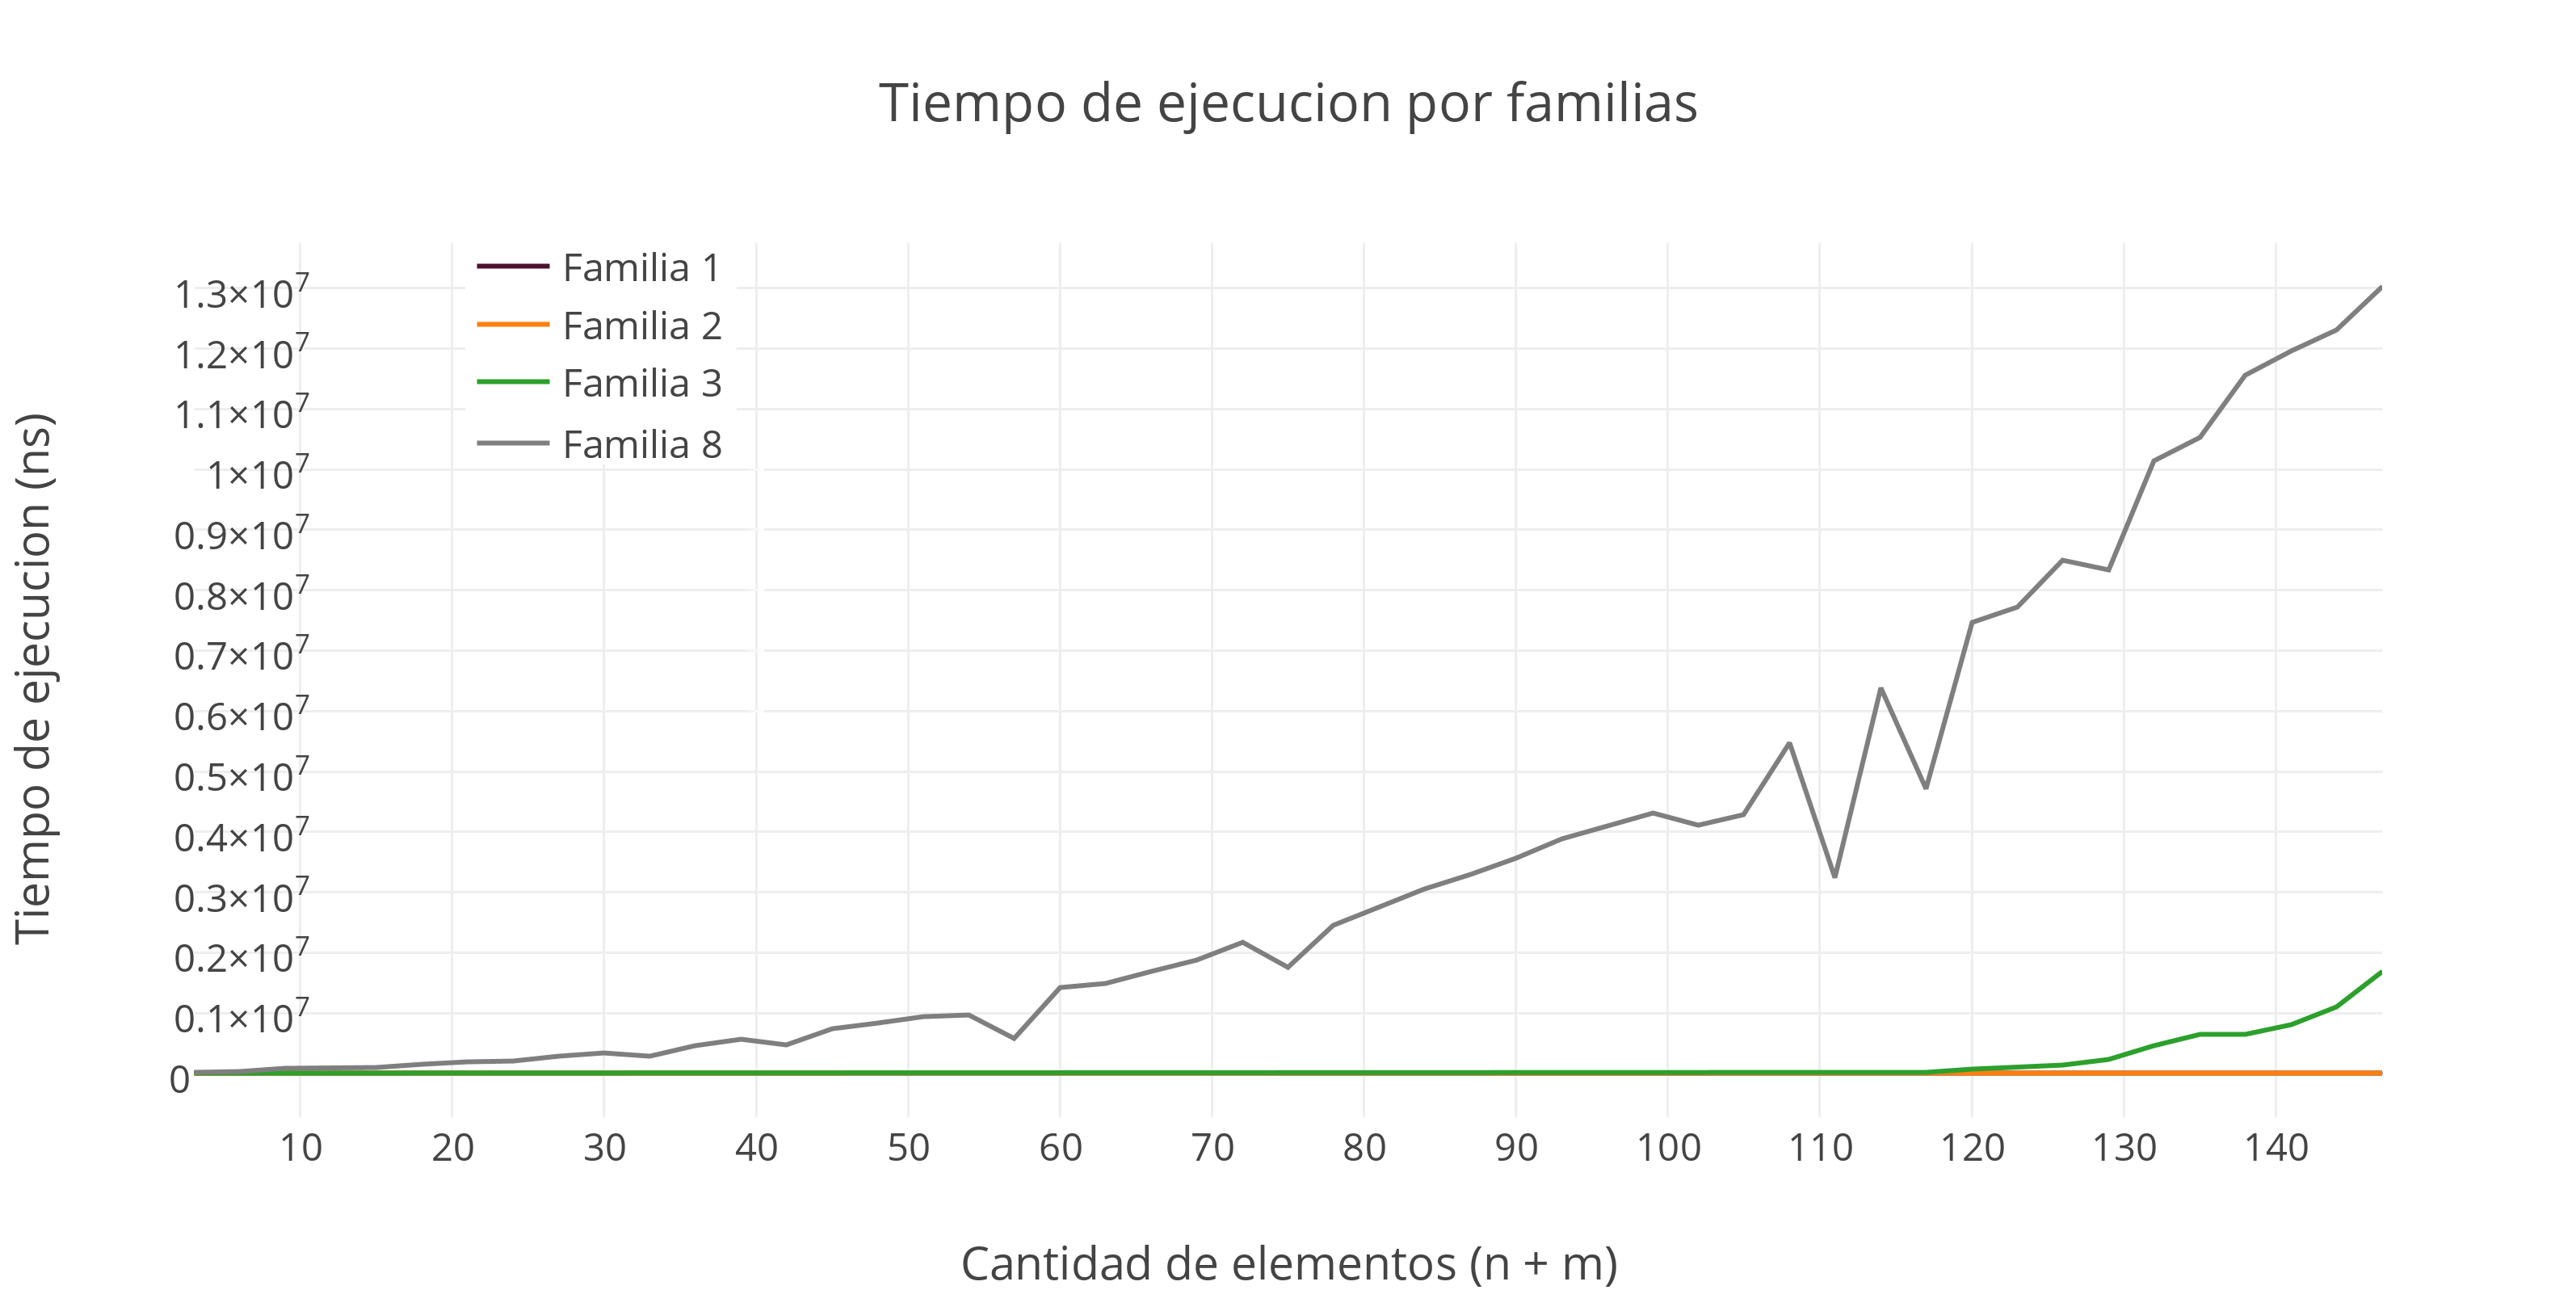
\includegraphics[width=0.45\textwidth]{./EJ2/comparativo2.png}}
    \label{fig:comparativo2}
    \end{figure}

Se puede observar como la familia n\'umero 6 presenta una peor performance en comparaci\'on al resto mientras que tanto la familia 1 como la 2 presentan un tiempo que se torna constante dando una mejor performance en relaci\'on al resto, lo cual se debe a las podas utilizadas para estas familias como mencionamos anteriormente. Mientras que la n\'umero 6 presenta la dificultad en la cual todos los elementos del mapa se encuentran desordenados, por lo tanto nuestro algoritmo tiene que llegar a hacer hasta un doble viaje para poder vencer a un gimnasio, ya que se dan instancias en las cuales los gimnasios de poder menor o igual a 3 se encuentran muy lejos de las pokeparadas en relaci\'on a los gimnasios de poder mayor, los cuales estan "pegados" a las pokeparadas insumiendo as\'i un tiempo mayor de decisi\'on y ejecuci\'on. Como hab\'iamos visto, nuestro algoritmo siempre que puede vencer a un gimnasio va a vencerlo.

Luego, mostraremos como se comporta nuestro algoritmo en base a la complejidad calculada anteriormente:

\vspace*{0.3cm} \vspace*{0.3cm}
  \begin{center}
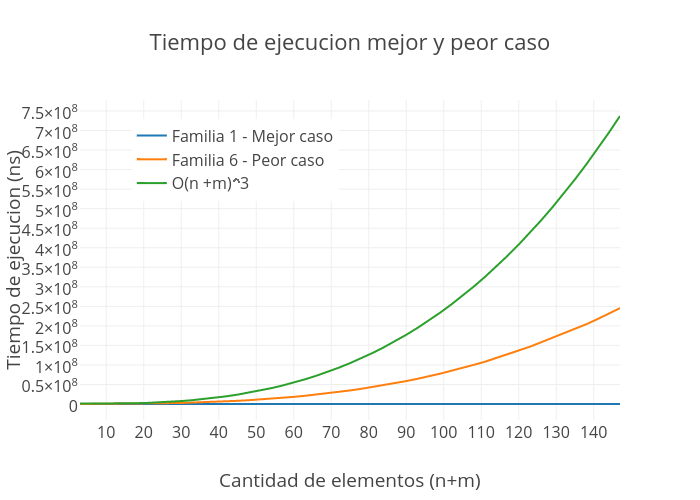
\includegraphics[scale=0.60]{./EJ2/mejorcaso.png}
\\{\textit{Tiempo de ejecución entre familias}}
  \end{center}
  \vspace*{0.3cm}

  
Es posible observar como las funciones resultantes del mejor y peor caso se encuentran por debajo de la cota de complejidad. Dicha complejidad fué calculada utilizando el m\'etodo de cuadrados m\'inimos generando una función que es tomada como cota dentro de nuestro orden de complejidad $(O(n+m)^3)$. 

--> INDICAR LA CONSTANTE: MELANIE LO PIDIO EL TEMA ES Q EL K NUESTRO ESTE ES UN NUMERO MEDIO TURBIO NO SE Q PONER.

\subsubsection{Familias random y Grupos de gimnasios}

Como se comentó previamente en el ejercicio uno, las anteriores familias fueron de utilidad para analizar que sucede con el algoritmo goloso dado cierto tipo de entradas y porque no obtiene solución óptima en algunos casos, además de servir para analizar las podas tanto del algorito exacto como el goloso. Lo que no fué posible con estas familias es analizar que sucede en el promedio de casos con soluciones aleatorias, dado que eran familias totalmente controladas para poder observar particularidades. Por este motivo introducimos aquí dos familias nuevas con el objetivo de analizar casos promedio dentro de conjuntos de un cierto tamaño.\\

La primera es la familia Random, que como el nombre lo indica, todo es absolutamente random en los parámetros de entrada.

La segunda familia también tiene parámetros aleatorios, pero organiza gimnasios por cuadrantes o grupos, donde $\forall$ $C_i$ con $i$ $\in$ ${1..4}$, todos los gimnasios en el cuadrante $C_j$ tienen el mismo poder. Otra regla que trató de aplicarse es que el poder de los gimnasios sea diferente para cada cuadrante $C_i$, $C_j$ con $i \neq j$. Esto será posible siempre y cuando no sea posible asignar m\'as de 1 (uno) de poder a los gimnasios, en cuyo caso, puede haber cuadrantes que tienen el mismo poder para sus gimnasios.

Esta familia será como una suerte de mapa por niveles. Veremos de esta manera como se desenvuelve sobre todo el algoritmo goloso para obtener un camino dentro de estas circunstancias.\\

Para el caso del valor de la mochila, con más de 15 elementos solo se analizará tomando el mínimo de mochila posible, y hasta con 15 elementos, podremos comparar contra el exacto que resulta de tomar la peor o la mejor mochila.
La mochila mínima será el valor del gimnasio con más poder más un extra de 3 ya que si el gimnasio más poderoso tiene valor menor a 3 podría generarse un caso sin solución. La mochila más grande será la suma de los poderes de todos los gimnasios. Mochilas con mayor tamaño harán que sobre capacidad.\\

Con respecto a la creación de casos para cada familia se idearon dos rangos iniciales:

\begin{enumerate}
\item Rango 1: de 5 a 20 elementos. Por cada instancia de tamaño $n$ se tomaron $n*5$ instancias aleatorias.
\item Rango 2: desde 70 hasta 470 elementos en intervalos de 50 elementos. Por cada instancia de tamaño $n$ se tomó un 10\% del tamaño de la entrada. 
\end{enumerate}

La cantidad de intancias dentro de cada tamaño será utilizada para promediar distancias y tiempos y así obtener errores relativos y porcentajes de mejora promedios por cada tamaño.\\

La idea del Rango 1 era poder calcular hasta con 20 elementos el backtracking, pero debido a los elevados tiempos de resolución se fué achicando el tamaño de las instancias hasta 15. Igualmente, por cuestiones de tiempo, se decidió conservar el rango de la manera en que fué ideado. La cantidad de instancias tomadas por cada tamaño permite obtener promedios más consistentes para que las comparaciones contra el backtracking sean de la mejor calidad posible y puedan aportar información sobre que es lo que sucede.

Para instancias mayores vale decir que intervalos de 50 elementos podría parecer ser demasiado, pero cuanto más se discretiza más tiempo de espera se necesita para correr todos los algoritmos que se verán en este informe. Como el objetivo principal es observar que sucede a medida que la entrada crece, se priorizó testear casos grandes resignando discretización. 

Ya que se decidió tomar intervalos de 50 elementos a partir de 20, el primer tamaño de entrada es 70. Puede observarse que un 10\% de 70 elementos son tan solo 7 elementos, pero aunque sea una cantidad pequeña, resultó ser igualmente buena para tomar promedios. Además, a medida que las instancias crecen en tamaño, el 10\% será una cantidad considerable de muestras generando buenos promedios para instancias grandes.

\newpage   

\subsubsection*{Repercusi\'on del tamaño de la mochila en el algoritmo hasta 15 elementos (pokeparadas + gimnasios)}

Se realizaron dos experimentas en base a la familia Random y a Grupos de gimnasios para ver como repercute el tamaño enunciado, con la mochila denominada grande y la chica. Luego de dicha experimentación, se desarrollaron los siguientes gr\'aficos en el cuales se podr\'a observar como la heur\'istica golosa no presenta cambios en su soluci\'on al tener una mochila mas grande o no, mientr\'as que el backtraking al tener una mochila con mayor capacidad logra obtener un camino diferente y de menor longitud.\\

\vspace*{0.3cm} \vspace*{0.3cm}
  \begin{center}
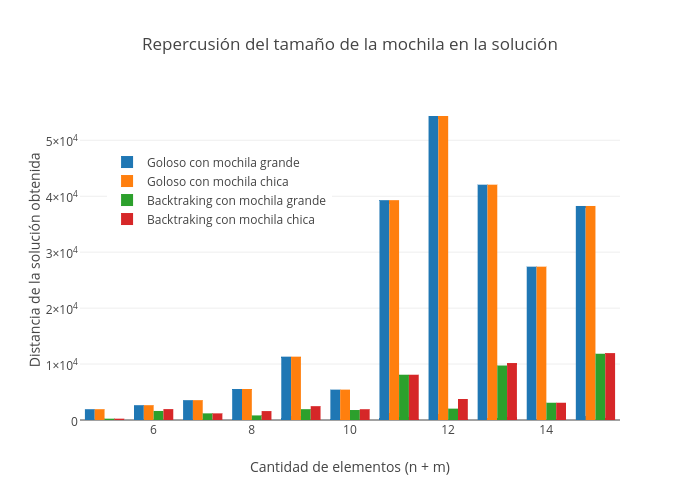
\includegraphics[scale=0.60]{./EJ2/familiaMochila.png}
\\{\textit{Grupos de gimnasios}}
  \end{center}
  \vspace*{0.3cm}
  \begin{figure} [h]
 \centering
  \subfloat[Repercusión en goloso]{
    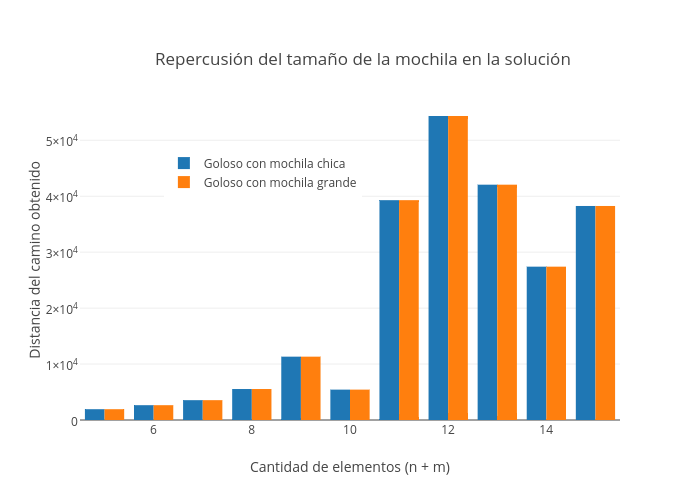
\includegraphics[width=0.45\textwidth]{./EJ2/mochilaGoloso.png}}
    \label{fig:comparativo1}
  \subfloat[Repercusión en backtraking]{
    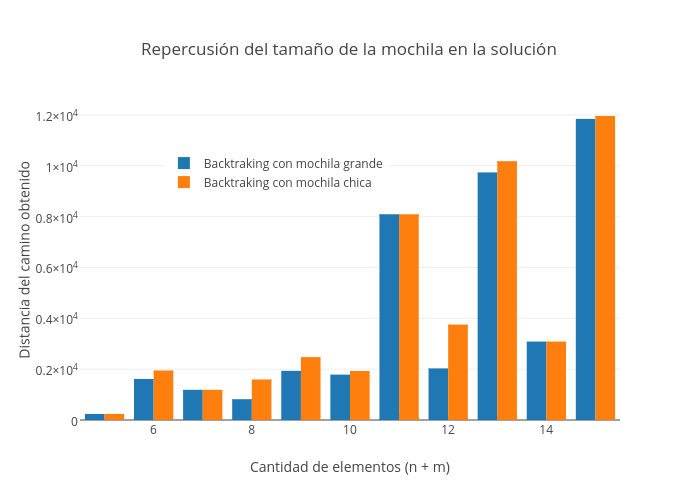
\includegraphics[width=0.45\textwidth]{./EJ2/mochilaBacktrakingFamilia.png}}
    \label{fig:comparativo2}
    \end{figure}
  
\vspace*{0.3cm} \vspace*{0.3cm}
  \begin{center}
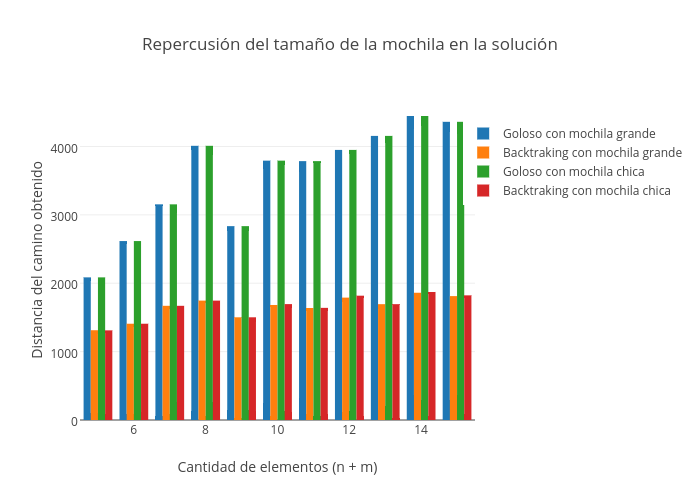
\includegraphics[scale=0.60]{./EJ2/randomMochila.png}
\\{\textit{Random}}
  \end{center}
  \vspace*{0.3cm}
  \begin{figure} [h]
 \centering
  \subfloat[Repercusión en goloso]{
    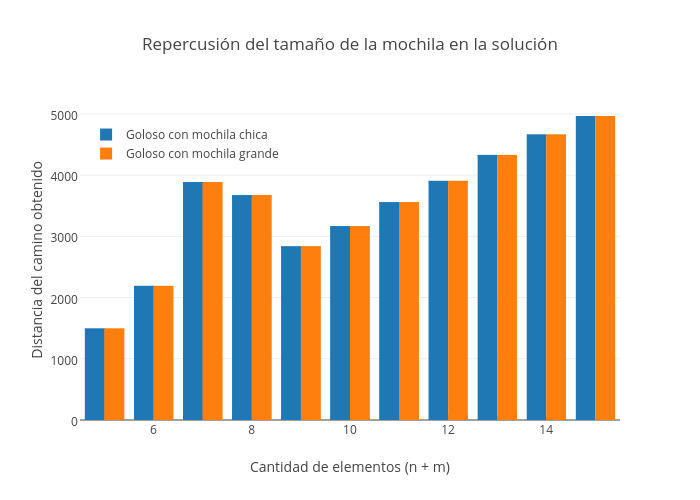
\includegraphics[width=0.45\textwidth]{./EJ2/mochilaGolosoRandom.png}}
    \label{fig:comparativo1}
  \subfloat[Repercusión en backtraking]{
    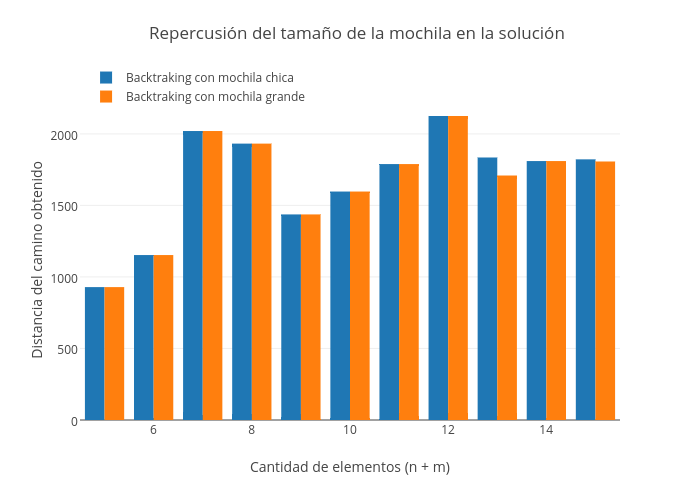
\includegraphics[width=0.45\textwidth]{./EJ2/mochilaBacktrakingRandom.png}}
    \label{fig:comparativo2}
    \end{figure}
   

Como se observa, en la heurística golosa no repercute el tamaño de la mochila, dado que la misma siempre que existe la posibilidad va a vencer a un gimnasio. Podemos notar sin embarlo algunas mejorías en cuanto a las mochilas grandes para los resultados del backtracking. Estos resultados tienen sentido. Ya que siempre se podrá obtener un resultado exacto mejor si se dispone de más capacidad de carga. Si hay las pokeparadas suficientes, con la mochila más grande posible podriamos primero cargar todas las pokeparadas necesarias y luego ir a vencer a todos los gimnasios. Si los gimnasios están lejos de todas las pokeparadas, esto termina beneficiando a la distancia recorrida ya que no será necesario volver a recargarse. 

\newpage

\subsubsection*{Repercusi\'on del tamaño de la mochila en el algoritmo más de 15 elementos}

Como se mencionó en repetidas oportunidades, al algoritmo goloso no saca partida de la capacidad de la mochila. Como con más de 15 elementos nos fué imposible calcular el backtracking en el ordenador disponible en tiempos razonables (no se llegó a terminar en una hora de corrida para 16 elementos), no podremos comparar que sucede al utilizar la peor y mejor mochila contra el resultado exacto.

\subsubsection*{Comparación de bactracking y algoritmo goloso para la familia Random}

\begin{figure} [h]
 \centering
  \subfloat[Algoritmo exacto]{
    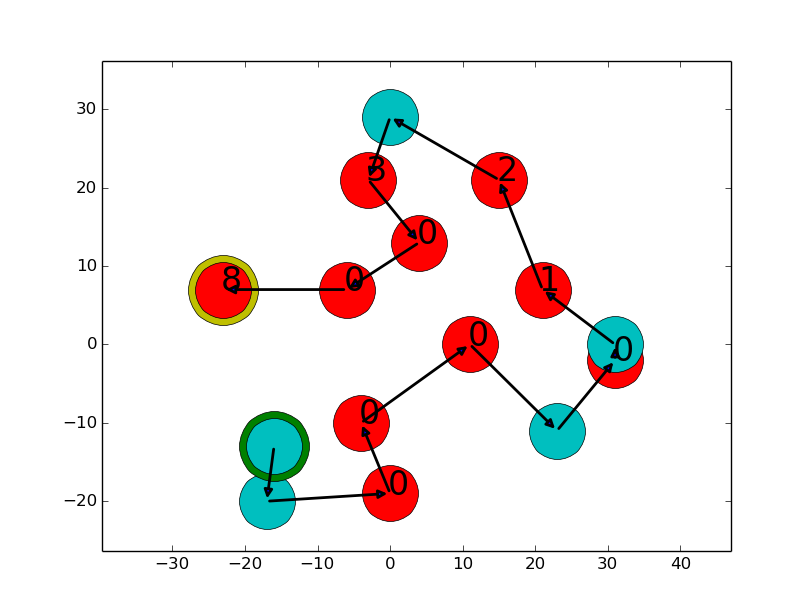
\includegraphics[width=0.45\textwidth]{./EJ2/randomexacto.png}}
       \label{fig:randomexacto}
  \subfloat[Algoritmo goloso]{
    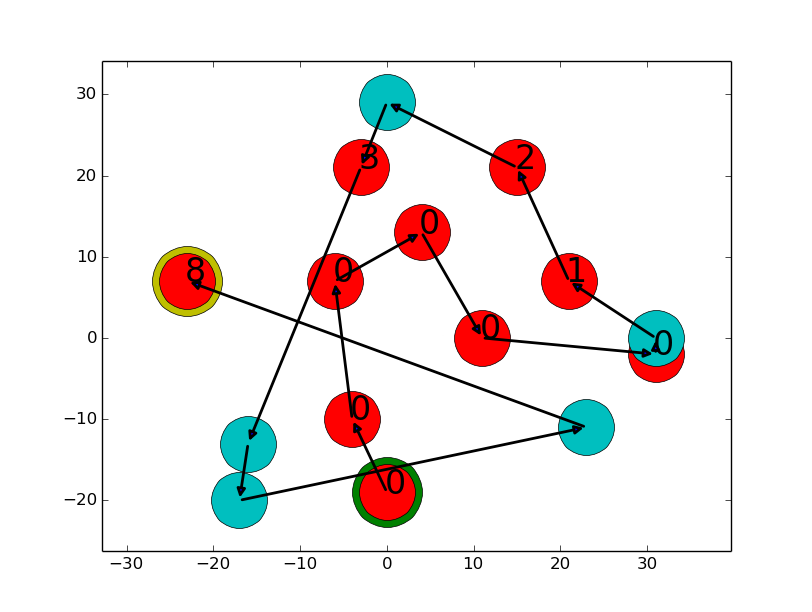
\includegraphics[width=0.45\textwidth]{./EJ2/randomgoloso.png}}
    \label{fig:randomgoloso}
    \end{figure}
 
Podemos ver a continuación la comparación entre soluciones obtenidas por ambos algoritmos:\\
 
\vspace*{0.3cm} \vspace*{0.3cm}
  \begin{center}
 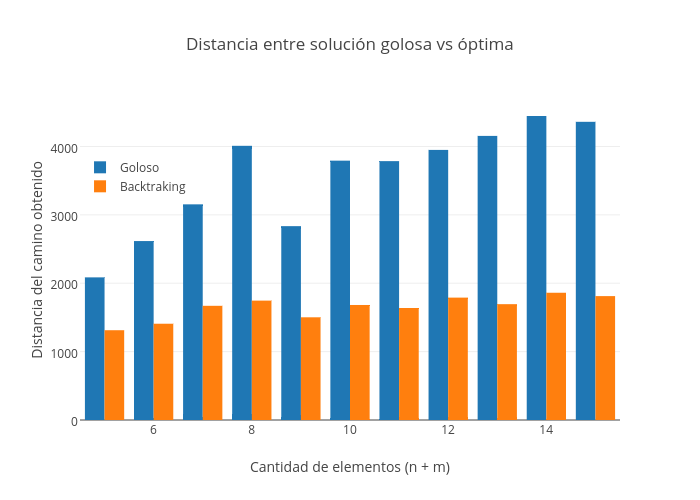
\includegraphics[width=0.75\textwidth]{./EJ2/random.png}
\\{\textit{Comparación solución golosa vs exacta}}
  \end{center}
  
     \vspace*{0.3cm} \vspace*{0.3cm}
  \begin{center}
 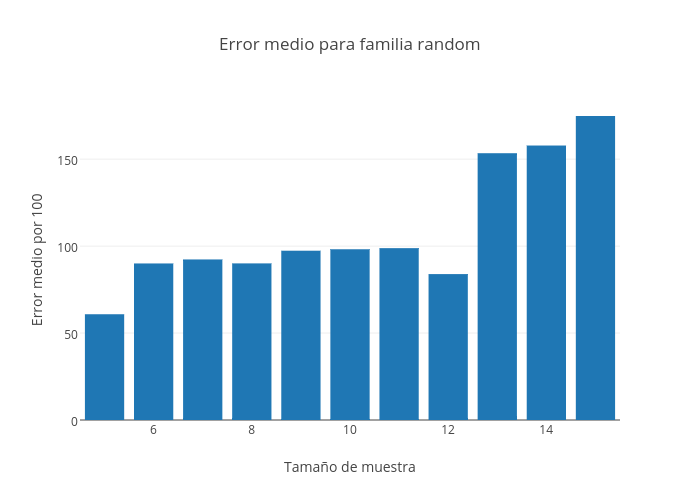
\includegraphics[width=0.75\textwidth]{./EJ2/randomError.png}
\\{\textit{Error relativo}}
\end{center}

Se observa para esta familia un error considerable cuanto más grande es la instancia, llegando a estar por arriba del 100\% con respecto al resultado exacto para entradas de 13 elementos. El motivo puede deberse a la variabilidad de los parámetros de entrada que hacen que el algoritmo goloso tenga que tomar las peores desiciones. Es decir, la mayoría de las veces se recorren grandes distancias para vencer a un gimnasio luego de juntar pokeparadas.

\subsubsection*{Comparación de bactracking y algoritmo goloso para la familia de Gimnasios por grupos} 

Podemos observar en las figuras el mismo mapa, donde (a) indica el recorrido exacto y (b) el recorrido goloso. Hay dos grupos de gimnasios. Un grupo con tres gimnasios de poder ocho y otro grupo con dos gimnasios de poder cero.

   \begin{figure} [h]
 \centering
  \subfloat[Algoritmo exacto]{
    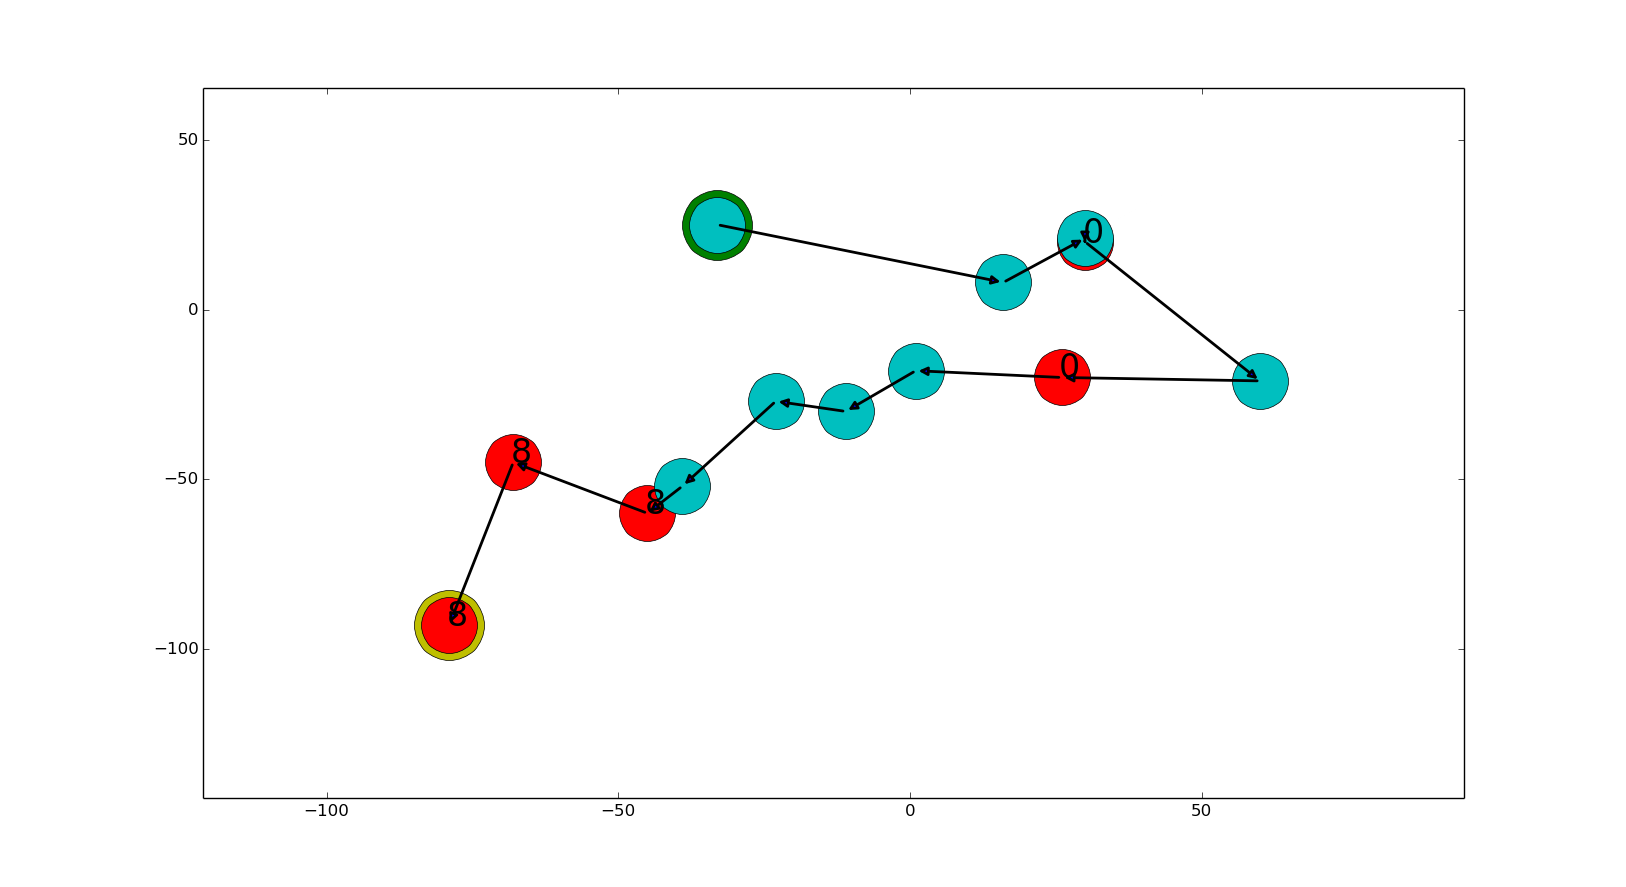
\includegraphics[width=0.45\textwidth]{./EJ2/familiaexacto.png}}
       \label{fig:randomexacto}
  \subfloat[Algoritmo goloso]{
    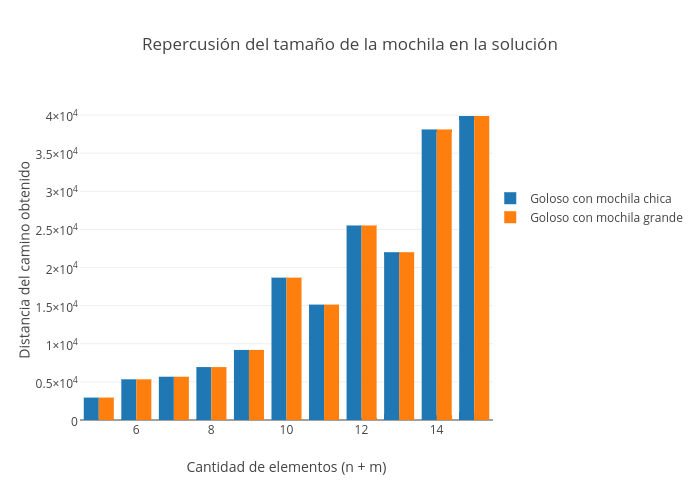
\includegraphics[width=0.45\textwidth]{./EJ2/familiaGoloso.png}}
    \label{fig:randomgoloso}
    \end{figure}
   
Con respecto a la diferencia entre la soluciones que se obtienen en relaci\'on a las \'optimas elebaramos los siguientes gráficos:\\
 
\vspace*{0.3cm} \vspace*{0.3cm}
  \begin{center}
 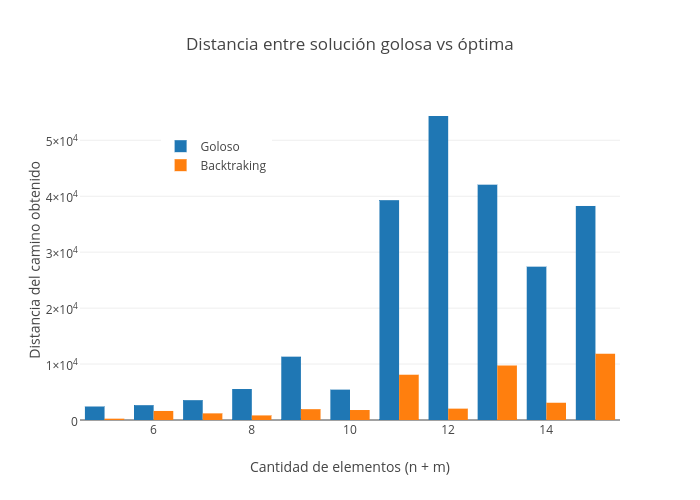
\includegraphics[width=0.75\textwidth]{./EJ2/familia.png}
\\{\textit{Comparación solución golosa vs exacta}}
  \end{center}

\vspace*{0.3cm} \vspace*{0.3cm}
  \begin{center}
 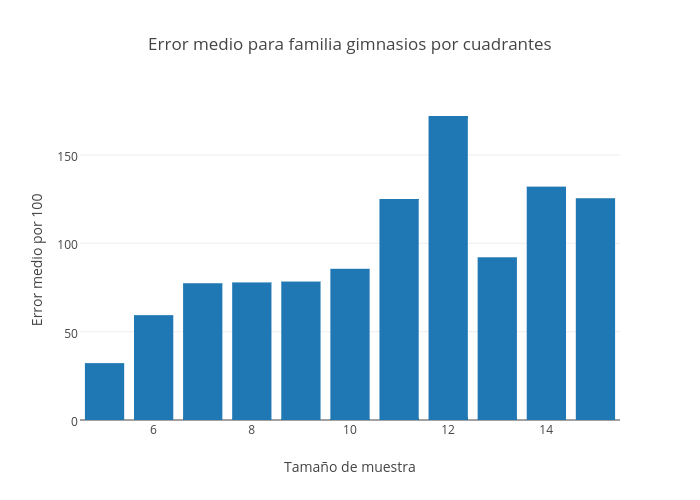
\includegraphics[width=0.75\textwidth]{./EJ2/familiaError.png}
\\{\textit{Error relativo}}
\end{center}

Podemos observar que habria que retestear tomando mas muestras!!

BOX: --->

\vspace*{0.3cm} \vspace*{0.3cm}
  \begin{center}
 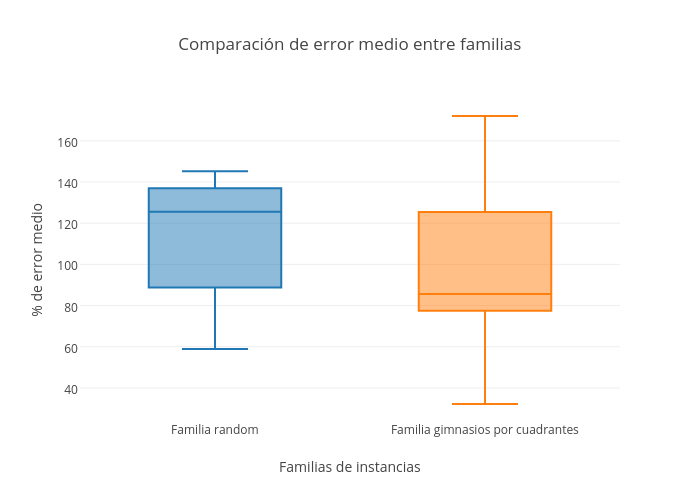
\includegraphics[width=0.75\textwidth]{./EJ2/box2.png}
\\{\textit{Errores absolutos por familia}}
\end{center}